% Options for packages loaded elsewhere
\PassOptionsToPackage{unicode}{hyperref}
\PassOptionsToPackage{hyphens}{url}
%
\documentclass[
  a4paper]{book}
\usepackage{lmodern}
\usepackage{amsmath}
\usepackage{ifxetex,ifluatex}
\ifnum 0\ifxetex 1\fi\ifluatex 1\fi=0 % if pdftex
  \usepackage[T1]{fontenc}
  \usepackage[utf8]{inputenc}
  \usepackage{textcomp} % provide euro and other symbols
  \usepackage{amssymb}
\else % if luatex or xetex
  \usepackage{unicode-math}
  \defaultfontfeatures{Scale=MatchLowercase}
  \defaultfontfeatures[\rmfamily]{Ligatures=TeX,Scale=1}
\fi
% Use upquote if available, for straight quotes in verbatim environments
\IfFileExists{upquote.sty}{\usepackage{upquote}}{}
\IfFileExists{microtype.sty}{% use microtype if available
  \usepackage[]{microtype}
  \UseMicrotypeSet[protrusion]{basicmath} % disable protrusion for tt fonts
}{}
\makeatletter
\@ifundefined{KOMAClassName}{% if non-KOMA class
  \IfFileExists{parskip.sty}{%
    \usepackage{parskip}
  }{% else
    \setlength{\parindent}{0pt}
    \setlength{\parskip}{6pt plus 2pt minus 1pt}}
}{% if KOMA class
  \KOMAoptions{parskip=half}}
\makeatother
\usepackage{xcolor}
\IfFileExists{xurl.sty}{\usepackage{xurl}}{} % add URL line breaks if available
\IfFileExists{bookmark.sty}{\usepackage{bookmark}}{\usepackage{hyperref}}
\hypersetup{
  pdftitle={BB512 - Population Biology and Evolution},
  pdfauthor={Owen R. Jones (Course Coordinator)},
  hidelinks,
  pdfcreator={LaTeX via pandoc}}
\urlstyle{same} % disable monospaced font for URLs
\usepackage{color}
\usepackage{fancyvrb}
\newcommand{\VerbBar}{|}
\newcommand{\VERB}{\Verb[commandchars=\\\{\}]}
\DefineVerbatimEnvironment{Highlighting}{Verbatim}{commandchars=\\\{\}}
% Add ',fontsize=\small' for more characters per line
\usepackage{framed}
\definecolor{shadecolor}{RGB}{248,248,248}
\newenvironment{Shaded}{\begin{snugshade}}{\end{snugshade}}
\newcommand{\AlertTok}[1]{\textcolor[rgb]{0.94,0.16,0.16}{#1}}
\newcommand{\AnnotationTok}[1]{\textcolor[rgb]{0.56,0.35,0.01}{\textbf{\textit{#1}}}}
\newcommand{\AttributeTok}[1]{\textcolor[rgb]{0.77,0.63,0.00}{#1}}
\newcommand{\BaseNTok}[1]{\textcolor[rgb]{0.00,0.00,0.81}{#1}}
\newcommand{\BuiltInTok}[1]{#1}
\newcommand{\CharTok}[1]{\textcolor[rgb]{0.31,0.60,0.02}{#1}}
\newcommand{\CommentTok}[1]{\textcolor[rgb]{0.56,0.35,0.01}{\textit{#1}}}
\newcommand{\CommentVarTok}[1]{\textcolor[rgb]{0.56,0.35,0.01}{\textbf{\textit{#1}}}}
\newcommand{\ConstantTok}[1]{\textcolor[rgb]{0.00,0.00,0.00}{#1}}
\newcommand{\ControlFlowTok}[1]{\textcolor[rgb]{0.13,0.29,0.53}{\textbf{#1}}}
\newcommand{\DataTypeTok}[1]{\textcolor[rgb]{0.13,0.29,0.53}{#1}}
\newcommand{\DecValTok}[1]{\textcolor[rgb]{0.00,0.00,0.81}{#1}}
\newcommand{\DocumentationTok}[1]{\textcolor[rgb]{0.56,0.35,0.01}{\textbf{\textit{#1}}}}
\newcommand{\ErrorTok}[1]{\textcolor[rgb]{0.64,0.00,0.00}{\textbf{#1}}}
\newcommand{\ExtensionTok}[1]{#1}
\newcommand{\FloatTok}[1]{\textcolor[rgb]{0.00,0.00,0.81}{#1}}
\newcommand{\FunctionTok}[1]{\textcolor[rgb]{0.00,0.00,0.00}{#1}}
\newcommand{\ImportTok}[1]{#1}
\newcommand{\InformationTok}[1]{\textcolor[rgb]{0.56,0.35,0.01}{\textbf{\textit{#1}}}}
\newcommand{\KeywordTok}[1]{\textcolor[rgb]{0.13,0.29,0.53}{\textbf{#1}}}
\newcommand{\NormalTok}[1]{#1}
\newcommand{\OperatorTok}[1]{\textcolor[rgb]{0.81,0.36,0.00}{\textbf{#1}}}
\newcommand{\OtherTok}[1]{\textcolor[rgb]{0.56,0.35,0.01}{#1}}
\newcommand{\PreprocessorTok}[1]{\textcolor[rgb]{0.56,0.35,0.01}{\textit{#1}}}
\newcommand{\RegionMarkerTok}[1]{#1}
\newcommand{\SpecialCharTok}[1]{\textcolor[rgb]{0.00,0.00,0.00}{#1}}
\newcommand{\SpecialStringTok}[1]{\textcolor[rgb]{0.31,0.60,0.02}{#1}}
\newcommand{\StringTok}[1]{\textcolor[rgb]{0.31,0.60,0.02}{#1}}
\newcommand{\VariableTok}[1]{\textcolor[rgb]{0.00,0.00,0.00}{#1}}
\newcommand{\VerbatimStringTok}[1]{\textcolor[rgb]{0.31,0.60,0.02}{#1}}
\newcommand{\WarningTok}[1]{\textcolor[rgb]{0.56,0.35,0.01}{\textbf{\textit{#1}}}}
\usepackage{graphicx}
\makeatletter
\def\maxwidth{\ifdim\Gin@nat@width>\linewidth\linewidth\else\Gin@nat@width\fi}
\def\maxheight{\ifdim\Gin@nat@height>\textheight\textheight\else\Gin@nat@height\fi}
\makeatother
% Scale images if necessary, so that they will not overflow the page
% margins by default, and it is still possible to overwrite the defaults
% using explicit options in \includegraphics[width, height, ...]{}
\setkeys{Gin}{width=\maxwidth,height=\maxheight,keepaspectratio}
% Set default figure placement to htbp
\makeatletter
\def\fps@figure{htbp}
\makeatother
\setlength{\emergencystretch}{3em} % prevent overfull lines
\providecommand{\tightlist}{%
  \setlength{\itemsep}{0pt}\setlength{\parskip}{0pt}}
\setcounter{secnumdepth}{-\maxdimen} % remove section numbering
\usepackage{booktabs}

\usepackage{tcolorbox}

\setlength{\fboxsep}{.8em}

\newtcolorbox{do-something}{
  colback=black!10!white,
  colframe=orange,
  coltext=black,
  boxsep=5pt,
  arc=4pt}

% \lstset{
%  breaklines=true
% }
\ifluatex
  \usepackage{selnolig}  % disable illegal ligatures
\fi

\title{BB512 - Population Biology and Evolution}
\author{Owen R. Jones (Course Coordinator)}
\date{2021-08-23}

\begin{document}
\frontmatter
\maketitle

\mainmatter
\hypertarget{welcome-to-bb512}{%
\chapter{Welcome to BB512}\label{welcome-to-bb512}}

Welcome to the Population and Evolution course. The course is divided
into two parts: Population and Evolution.

The population part comes first and covers ecological population
dynamics including models of population growth, species interactions,
and other demographic models.

The recommended textbook is: Gotelli, NJ (2008) \emph{A Primer of
Ecology}. Fourth Edition, Sinauer Associates. ISBN: 978-0878933181

The evolution part comes second and covers microevolutionary processes
(natural selection, neutral evolution etc.), population and quantitative
genetics, and macroevolution (speciation, extinction and coevolution).

The recommended textbook is: Stearns, SC \& Hoekstra, RF (2005)
\emph{Evolution: An Introduction}. 2nd Edition, Oxford University Press.
ISBN: 978-0199255634

\hypertarget{this-website-and-other-course-materials}{%
\section{This website and other course
materials}\label{this-website-and-other-course-materials}}

This website is designed to hold most of the materials you need for the
practical (mainly computer) exercises you will do during the course. You
will also find the
\href{https://jonesor.github.io/BB512_Book/schedule.html}{Schedule}
here.

You will find other materials via itsLearning. Apart from the book,
there will be some recommended scientific papers to read -- these will
be accessible via links on itsLearning.

In some of the classes there will be exercises conducted on your
personal laptops. Please bring them to class (and remember a power
supply!).

\hypertarget{expectations}{%
\section{Expectations}\label{expectations}}

There are lectures and exercise sessions on the course. The exercise
sessions are designed to help you understand the subject better and I
expect students to attend and actively participate in both. There will
also be some e-tests throughout the semester. These are intended to help
you figure out whether you know the material, and whether there are
areas you need to revisit. They do not contribute to your final grade,
but I hope you will attempt them. They will definitely increase your
understanding of the material! Note that the final assessment will be a
similar format!

I also expect students to make every effort to keep up with the core
reading (mainly the textbook chapters), and to ask questions where they
don't understand.

\hypertarget{your-feedback}{%
\section{Your feedback}\label{your-feedback}}

I would really like your feedback on how the course is progressing so I
can address any issues that come up as soon as possible. To help with
this I have created a simple Google Form: \url{http://goo.gl/gy2Q6B}.
You can use this to send me (Owen) comments (anonymously if you wish) at
any time in the course. I promise to do my best to resolve any problems.

\hypertarget{assessment}{%
\section{Assessment}\label{assessment}}

The assessment for the course will be an electronic exam held next
January with multiple choice and short answer questions. It is worth
noting that exam format will be similar to the quizzes mentioned above.
The exact date is not yet set.

\hypertarget{instructors}{%
\section{Instructors}\label{instructors}}

The instructors of the course are:

\begin{itemize}
\tightlist
\item
  \href{https://portal.findresearcher.sdu.dk/en/persons/jones}{Owen
  Jones}, Associate Professor,
  \href{mailto:jones@biology.sdu.dk}{\nolinkurl{jones@biology.sdu.dk}}
\item
  \href{https://portal.findresearcher.sdu.dk/en/persons/thomasbb}{Thomas
  Bjørneboe Berg}, Associate Prof./Senior Scientist at Naturama,
  \href{mailto:thomas@naturama.dk}{\nolinkurl{thomas@naturama.dk}}
\end{itemize}

Finally, if you have any problems accessing materials, or have any
questions regarding the course feel free to send me an email, or make a
comment in the form I mentioned above. You can also make an appointment
to see me via Zoom or in my office if necessary*.

Owen Jones, course coordinator -
\href{mailto:jones@biology.sdu.dk}{\nolinkurl{jones@biology.sdu.dk}}

Office location:
\href{https://clients.mapsindoors.com/sdu/573f26e4bc1f571b08094312/details/563cb94f423b7d0540c9a605}{V12-410b-2}

\begin{do-something}
\textbf{Note:} The website is an experimental ``work in progress'' and
will change during the course as I add material. The latest version can
always be found at the website.

Please let me know
(\href{mailto:jones@biology.sdu.dk}{\nolinkurl{jones@biology.sdu.dk}})
if you spot any errors, or have any suggestions for improvement.
\end{do-something}

\hypertarget{schedule}{%
\chapter{Schedule}\label{schedule}}

This is the schedule for the course. Please note that it is liable to
change (possibly at short notice). If you find a mismatch between this
schedule and the official one\footnote{\url{https://mitsdu.sdu.dk/skema/activity/N100007101/e21}},
then it is the official one that is correct.

The \emph{Textbook} column tells you the chapter(s) of the two textbooks
that are most relevant to the session. The two textbooks are Gotelli
(G)\footnote{ Gotelli, NJ (2008) \emph{A Primer of Ecology}. Fourth
  Edition, Sinauer Associates. ISBN: 978-0878933181} and Stearns and
Hoekstra (SH)\footnote{Stearns, SC \& Hoekstra, RF (2005)
  \emph{Evolution: An Introduction}. 2nd Edition, Oxford University
  Press. ISBN: 978-0199255634}, and the numbers refer to the chapter
numbers (e.g.~SH.3, means Chapter 3 in Stearns and Hoekstra).

You should aim to read these chapters as the course proceeds.

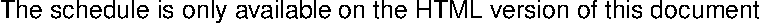
\includegraphics{BB512_files/figure-latex/unnamed-chunk-4-1.pdf}

\hypertarget{part-population-biology}{%
\chapter*{(PART) Population Biology}\label{part-population-biology}}
\addcontentsline{toc}{chapter}{(PART) Population Biology}

\hypertarget{the-legend-of-ambalapuzha}{%
\chapter{The legend of Ambalapuzha}\label{the-legend-of-ambalapuzha}}

Exponential growth is a powerful concept. To help us grasp it better
lets use an ancient Indian chess legend as an example.

\begin{center}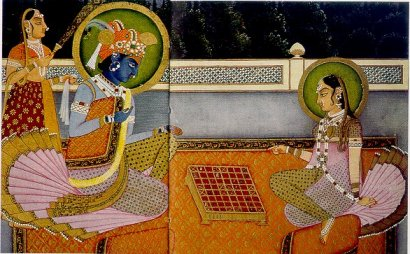
\includegraphics[width=0.5\linewidth]{images/Radha-Krishna_chess} \end{center}

According to legend, Lord Krishna once appeared in the form of a wise
man in the court of the king and challenged him to a game of chess. The
king was a chess enthusiast and naturally accepted the invitation.

The king asked the wise man to choose a prize in case he won. The old
man told the king that he had few material needs and that all he wished
was a few grains of rice.

He added that the amount of rice itself should be determined using the
chess- board in the following manner: one grain of rice would be placed
in the first square, two grains in the second square, four in the third
square, and so on. Every square would have double the number of grains
of its predecessor.

Upon hearing this, the king was unhappy, since the man requested only a
few grains of rice instead of any of the other riches of the kingdom,
which the king would have been happy to donate (he was a generous guy).
He requested the old man to add other items to his prize, but the man
declined.

So the game of chess started and, needless to say, the king lost the
game so it was soon time to pay the old man his prize. As he started
adding grains of rice to the chessboard, the king soon realised the true
nature of the wise man's demand. The royal granary soon ran out of rice
and the king realised that even if he provided all the rice in his
kingdom and even the whole of India, he would never be able to fulfill
the promised reward. He was distraught that he could not fulfill his
promise!

Seeing the king upset, the wise man appeared to the king in his true
form, that of Lord Krishna. He told the king that he did not have to pay
the debt immediately but could pay him over time. The king would serve
rice in the temple freely to the pilgrims every day until the debt was
paid off. And that is why the Ambalappuzha Temple in India still serves
rice to pilgrims -- the debt is still being paid off.

\begin{do-something}
Use the Excel sheet
(\texttt{{[}RiceOnAChessboard.xlsx{]}(https://www.dropbox.com/s/nf81t0hzz34vyzk/RiceOnAChessboard.xlsx?dl=1)})
to calculate the quantity of rice that the king owed.

A grain of rice weighs 25mg, what weight of rice did the king owe in
total, in kg?
\end{do-something}

\hypertarget{animalsplants-not-grains-of-rice.}{%
\section{Animals/plants, not grains of
rice.}\label{animalsplants-not-grains-of-rice.}}

Imagine that instead of rice, we were talking about the population
growth of bacteria, or rabbits, reproducing every time step.

\begin{itemize}
\tightlist
\item
  Would the model be realistic?
\item
  Why/why not?
\item
  What other factors should be taken into account?
\end{itemize}

\hypertarget{optional-try-these-calculations-in-r}{%
\section{Optional: Try these calculations in
R}\label{optional-try-these-calculations-in-r}}

You can do this kind of calculation easily in \emph{R}. Try this.

\begin{Shaded}
\begin{Highlighting}[]
\NormalTok{myData }\OtherTok{\textless{}{-}} \FunctionTok{data.frame}\NormalTok{(}\AttributeTok{Squares =} \DecValTok{1}\SpecialCharTok{:}\DecValTok{64}\NormalTok{,}\AttributeTok{nRice =} \ConstantTok{NA}\NormalTok{)}
\NormalTok{myData}\SpecialCharTok{$}\NormalTok{nRice[}\DecValTok{1}\NormalTok{] }\OtherTok{\textless{}{-}} \DecValTok{1} 

\ControlFlowTok{for}\NormalTok{ (i }\ControlFlowTok{in} \DecValTok{2}\SpecialCharTok{:}\DecValTok{64}\NormalTok{)\{}
\NormalTok{  myData}\SpecialCharTok{$}\NormalTok{nRice[i] }\OtherTok{\textless{}{-}}\NormalTok{ myData}\SpecialCharTok{$}\NormalTok{nRice[i}\DecValTok{{-}1}\NormalTok{]}\SpecialCharTok{*}\DecValTok{2}
\NormalTok{\}}
\end{Highlighting}
\end{Shaded}

Now we can look at the top and bottom of the 64 row data frame like
this:

\begin{Shaded}
\begin{Highlighting}[]
\FunctionTok{head}\NormalTok{(myData)}
\end{Highlighting}
\end{Shaded}

\begin{verbatim}
##   Squares nRice
## 1       1     1
## 2       2     2
## 3       3     4
## 4       4     8
## 5       5    16
## 6       6    32
\end{verbatim}

\begin{Shaded}
\begin{Highlighting}[]
\FunctionTok{tail}\NormalTok{(myData)}
\end{Highlighting}
\end{Shaded}

\begin{verbatim}
##    Squares        nRice
## 59      59 2.882304e+17
## 60      60 5.764608e+17
## 61      61 1.152922e+18
## 62      62 2.305843e+18
## 63      63 4.611686e+18
## 64      64 9.223372e+18
\end{verbatim}

And we can sum up the total number of grains of rice on the 64 squares
of the board like this:

\begin{Shaded}
\begin{Highlighting}[]
\FunctionTok{sum}\NormalTok{(myData}\SpecialCharTok{$}\NormalTok{nRice)}
\end{Highlighting}
\end{Shaded}

\begin{verbatim}
## [1] 1.844674e+19
\end{verbatim}

To put that \emph{HUGE} number in context, if a grain of rice ways 25mg
(0.0000025kg), then we'd have 46,116,860,184,274 kg.

\hypertarget{geometric-growth}{%
\chapter{Geometric growth}\label{geometric-growth}}

In a simple model of population growth where the population grows
without any constraints, the speed a population increases in size can be
described by the population growth rate. This is often given by the
symbol lambda (\(\lambda\)). High values of \(\lambda\) mean the
population grows fast, while small values indicated that it grows
slowly, or shrinks in size.

Geometric growth is often seen as synonymous to exponential growth. It
basically is, but with one important difference: exponential growth,
strictly speaking, refers to ``continuous time'' scenarios, whereas
geometric growth refers to models where the population changes in
discrete time steps (e.g.~each year).

Download and open the Excel file
\href{https://www.dropbox.com/s/xxx05sckvop5i52/GeometricGrowth.xlsx?dl=1}{\texttt{GeometricGrowth.xlsx}}.

\begin{enumerate}
\def\labelenumi{\arabic{enumi}.}
\tightlist
\item
  Starting with an initial population size (\texttt{N}) of 10 {[}at time
  (\texttt{t}) =0{]}, and with a \(\lambda\) of \texttt{1.1}, use
  Excel's equation functions to work out the population size from
  \texttt{t=1} through to \texttt{t=20}. E.g. The formula might look
  something like this ``\texttt{=B8*\$F\$8}.''
\item
  Use charts to plot the results. On the horizontal axis (x-axis) you
  should have time, and on the vertical axis (y-axis) you should have
  population size (\texttt{N}). A scatterplot would be best for this.
\item
  Make another plot of the same data, but this time use a natural
  logarithmic axis for the population size. The formula in Excel for
  natural log is \texttt{LN()}.
\item
  What do you notice about the curves in these different versions of
  plotting the same data?
\item
  Try altering the population growth rate. Try values of 0.8, 1 and 1.2
  for example. What happens to the curves? What is special about the
  value of 1?
\end{enumerate}

Now reset the population growth rate to 1.1. Now lets see if the
mathematical rules of so-called ``geometric series'' work\ldots{}

\begin{enumerate}
\def\labelenumi{\arabic{enumi}.}
\tightlist
\item
  If the population starts at t=0, \(N_t = N_0 \lambda^t\) . In words,
  the population at time \(t\) is the initial population size multiplied
  by the finite population growth rate raised to the power of \(t\).
\item
  Your instructor will explain how this works on the blackboard.
\item
  Following these rules, the population size at time \(t=5\) (\(N_5\)),
  is \(10 * 1.1^5\), or \(10* 1.61051\), which is \(16.1051\). Check
  that this matches what you got earlier.
\item
  This approach can be really useful because it can save lots of time.
  For example, what is the population after 900 generations? It would be
  tedious to work this out using the first, ``simple'' approach, but
  very easy if you use the geometric series rules.
\end{enumerate}

\hypertarget{stochastic-population-growth}{%
\chapter{Stochastic population
growth}\label{stochastic-population-growth}}

We will examine the effect of adding stochasticity (randomness) into the
simple exponential/geometric growth model you have been looking at in
the last couple of lectures. Remember -- this model allows for unbounded
population growth -- the populations development is not influenced by
population density.

We'll focus on the discrete form: \(N_{t+1}=λN_t\)\footnote{Equation
  1.15 in Gotelli}

In many cases it is unlikely that the finite rate of increase (\(λ\))
will be constant through time. Population growth rates are likely to
vary through time because of environmental factors (weather, food supply
etc.). This is called \emph{environmental stochasticity}.

We will create some models in Excel, and in R, to explore the effect
that this variation has.

A good way to begin thinking about this topic is to consider that the
instantaneous rate of increase (\(r\)) of the population can vary. We
can simulate this by drawing a random number drawn from a normal
distribution with a mean (\(\bar{r}\)) and variance (\(\sigma_r^2\))
(Fig. @ref(fig:stochGrowthRate)). In the figure you can see that the
peak of the \(r\) distribution is \(>0\) (approximately 0.1), so on
average, the population will tend to grow. However, in poor years \(r\)
is \(<\) 0, so the population will decline in those cases. Both the mean
value and the spread of the distribution (i.e.~variance or standard
deviation) determine the fate of the population. We can convert \(r\) to
\(\lambda\) by taking the exponential, because
\(r = ln(\lambda)\)\footnote{equation 1.5 in Gotelli}

\begin{figure}

{\centering 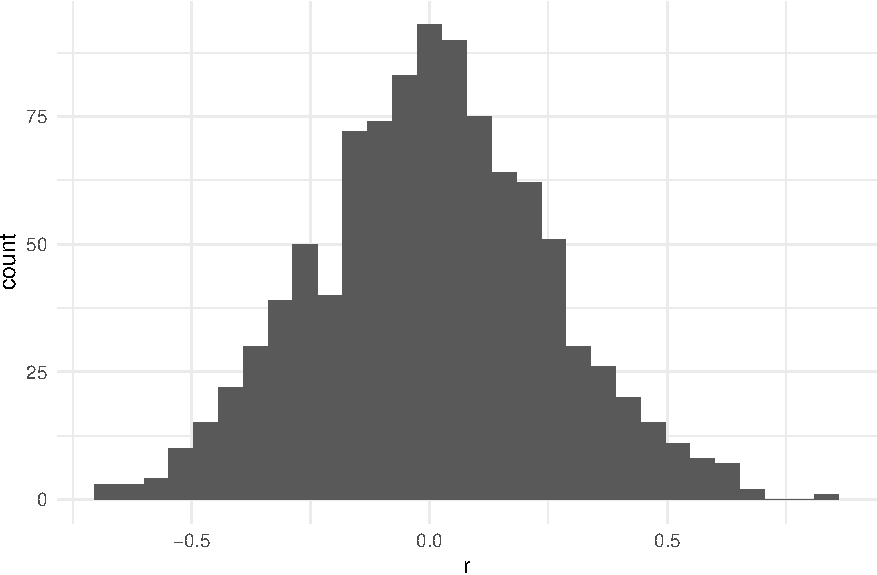
\includegraphics{BB512_files/figure-latex/stochGrowthRate-1} 

}

\caption{A normal distribution of potential r values}\label{fig:stochGrowthRate}
\end{figure}

When using the equation above to calculate population at time \(t+1\)
(\(N_{t+1}\)) from the population at time \(t\) (\(N_t\)), one would
draw a random \(r\) value from this distribution. Sometimes \(r\) will
be high, other times it will be low, most of the time it will be from
around the middle of the distribution.

\begin{do-something}
Use the Excel worksheet,
\texttt{{[}StochasticPopulationGrowth.xslx{]}(https://www.dropbox.com/s/1wpixbpgwlh54f0/StochasticPopulationGrowth.xlsx?dl=1)},
to study how stochastic population growth works with this simple model.
\end{do-something}

\begin{enumerate}
\def\labelenumi{\arabic{enumi})}
\tightlist
\item
  Use Excel formulae to calculate deterministic population size through
  time (20 generations, with starting population of 100), linking to the
  mean finite population growth rate.
\item
  Use charts to plot the results. (you already did this last time!)
\item
  Use a formula to generate a column of stochastic \(r\) values, based
  on a particlar mean and variance. {[}English Excel:
  \texttt{=NORMINV(RAND(),\$F\$10,SQRT(\$F\$11))}/ Danish Excel:
  \texttt{=NORMINV(SLUMP();\$F\$10;KVROD(\$F\$11))}. If you get errors,
  check whether Excel is expecting commas or semi-colons{]}
\item
  Use the same procedure as before, to create a stochastic population
  size vector (stochastic N). Remember to convert \(r\) to \(\lambda\)
  by taking the exponential.
\item
  Compare the two trajectories using a chart.
\item
  Try altering initial population size, the mean finite growth rate, and
  the amount of stochasticity (Variance).
\item
  Extinction occurs when N \(\leq\) 0. What happens to extinction risk
  as stochasticity increases? What hapens when initial N is small?
\end{enumerate}

\begin{do-something}
Note: Excel re-randomises the random numbers every time you change any
cell in the sheet. This is OK, and allows you to explore a stochastic
simulation many times.
\end{do-something}

\hypertarget{simulations-in-r}{%
\section{Simulations in R}\label{simulations-in-r}}

Excel is of limited use to really get a feel for this. For the next part
we'll use \emph{R}.

If you already have R on your computers you can play along, otherwise
take a look at my demonstration in class. I will show how you can use
this simulation approach to estimate extinction risk and how this is
related to starting population size, mean lambda, and the amount of
stochasticity.

You can copy/paste the code below into \emph{R}.

The output of the modelling is shown in Fig. @ref(fig:stochProjection)

\begin{do-something}
Copy-and-paste the code below into a text file (or directly into
\emph{R}).

The final line of the code (\texttt{nExtinct/nTrials}) gives you an
estimate of extinction probability - the proportion of trials that lead
to a population size of 1 (or less).

Modify the simulation settings to explore what happens to (i) the plot
of population growth and (ii) extinction risk, when you vary
\texttt{mean.r} (\(\bar{r}\)), the amount of stochasticity
(\(\sigma_r^2\)) (\texttt{var.r}), and the number of generations
(\texttt{nGen}).
\end{do-something}

\begin{Shaded}
\begin{Highlighting}[]
\CommentTok{\#Simulating stochastic geometric population growth rate}

\CommentTok{\#Simulation settings (try changing these)}
\NormalTok{mean.r }\OtherTok{=} \FloatTok{0.05} \CommentTok{\# the mean value of r}
\NormalTok{var.r }\OtherTok{=} \FloatTok{0.1} \CommentTok{\# the variance in r (stochasticity)}
\NormalTok{startPop }\OtherTok{=} \DecValTok{10} \CommentTok{\# pop size at start}
\NormalTok{nGen }\OtherTok{=} \DecValTok{50} \CommentTok{\# number of generations}
\NormalTok{nTrials }\OtherTok{=} \DecValTok{100} \CommentTok{\# number of repeated simulations}

\DocumentationTok{\#\#\#\#\#\#\#\#\#\#\#\#\#\#\#\#\#\#\#\#\#\#\#\#\#\#\#\#\#\#\#\#\#\#\#\#\#\#\#\#\#\#\#\#\#\#\#\#\#\#\#\#\#\#\#\#\#\#\#\#\#\#\#\#\#\#\#\#}
\CommentTok{\#If you are unfamiliar with R, do not edit anything below this line!}
\DocumentationTok{\#\#\#\#\#\#\#\#\#\#\#\#\#\#\#\#\#\#\#\#\#\#\#\#\#\#\#\#\#\#\#\#\#\#\#\#\#\#\#\#\#\#\#\#\#\#\#\#\#\#\#\#\#\#\#\#\#\#\#\#\#\#\#\#\#\#\#\#}

\NormalTok{pseudoExtinction }\OtherTok{=} \DecValTok{1}

\CommentTok{\# First randomly generate some lambda values}
\NormalTok{rValues}\OtherTok{\textless{}{-}}\FunctionTok{matrix}\NormalTok{(}\FunctionTok{rnorm}\NormalTok{(nTrials}\SpecialCharTok{*}\NormalTok{nGen, }\AttributeTok{mean =}\NormalTok{ mean.r, }\AttributeTok{sd =} \FunctionTok{sqrt}\NormalTok{(var.r)),}\AttributeTok{ncol=}\NormalTok{nTrials,}\AttributeTok{nrow=}\NormalTok{nGen)}

\CommentTok{\# Use a histogram to see what they look like (uncomment the line below)}
\CommentTok{\# hist(lambdas,col="grey",main="")}

\CommentTok{\# Now run the simulations to see what the resulting population growth looks like}
\NormalTok{trials }\OtherTok{=} \FunctionTok{matrix}\NormalTok{(}\AttributeTok{data =} \ConstantTok{NA}\NormalTok{, }\AttributeTok{nrow =}\NormalTok{ nGen, }\AttributeTok{ncol =}\NormalTok{ nTrials)}
\ControlFlowTok{for}\NormalTok{ (j }\ControlFlowTok{in} \DecValTok{1}\SpecialCharTok{:}\NormalTok{nTrials)\{}
\NormalTok{  popSize }\OtherTok{=}\NormalTok{ startPop  }
  \ControlFlowTok{for}\NormalTok{ (i }\ControlFlowTok{in} \DecValTok{2}\SpecialCharTok{:}\NormalTok{ nGen)\{}
\NormalTok{  stoch.r }\OtherTok{=}\NormalTok{ rValues[i,j]}
\NormalTok{  popSize }\OtherTok{=} \FunctionTok{append}\NormalTok{(popSize, popSize[i}\DecValTok{{-}1}\NormalTok{]}\SpecialCharTok{*}\FunctionTok{exp}\NormalTok{(stoch.r))}
\NormalTok{\}}
\NormalTok{trials[,j] }\OtherTok{=}\NormalTok{ popSize}
\FunctionTok{rm}\NormalTok{(popSize)}
\NormalTok{\}}

\CommentTok{\#Calculate probability of (pseudo)extinction}
\NormalTok{minvals }\OtherTok{\textless{}{-}} \FunctionTok{apply}\NormalTok{(trials,}\DecValTok{2}\NormalTok{,min)}
\NormalTok{nExtinct }\OtherTok{\textless{}{-}} \FunctionTok{length}\NormalTok{(minvals[minvals}\SpecialCharTok{\textless{}=}\NormalTok{pseudoExtinction])}
\NormalTok{nExtinct}\SpecialCharTok{/}\NormalTok{nTrials}
\end{Highlighting}
\end{Shaded}

\begin{verbatim}
## [1] 0.08
\end{verbatim}

\begin{Shaded}
\begin{Highlighting}[]
\CommentTok{\#Make a plot of the population trajectories}
\FunctionTok{plot}\NormalTok{(}\DecValTok{1}\SpecialCharTok{:}\NormalTok{nGen,}\FunctionTok{log}\NormalTok{(}\FunctionTok{seq}\NormalTok{(}\FloatTok{0.1}\NormalTok{,}\FunctionTok{max}\NormalTok{(trials),}\AttributeTok{length.out=}\NormalTok{nGen)),}\AttributeTok{type =} \StringTok{"n"}\NormalTok{,}\AttributeTok{axes=}\NormalTok{F,}\AttributeTok{xlab =}\StringTok{"Time"}\NormalTok{, }\AttributeTok{ylab =} \StringTok{"N"}\NormalTok{,}\AttributeTok{ylim=}\FunctionTok{log}\NormalTok{(}\FunctionTok{c}\NormalTok{(}\FloatTok{0.1}\NormalTok{,}\DecValTok{100000}\NormalTok{)))}
\FunctionTok{matlines}\NormalTok{(}\FunctionTok{log}\NormalTok{(trials),}\AttributeTok{col =} \StringTok{"\#FF234520"}\NormalTok{,}\AttributeTok{lty=}\DecValTok{1}\NormalTok{,}\AttributeTok{lwd=}\DecValTok{3}\NormalTok{)}
\FunctionTok{axis}\NormalTok{(}\DecValTok{1}\NormalTok{)}
\FunctionTok{axis}\NormalTok{(}\DecValTok{2}\NormalTok{,}\AttributeTok{at =} \FunctionTok{log}\NormalTok{(}\FunctionTok{c}\NormalTok{(}\FloatTok{0.1}\NormalTok{,}\DecValTok{1}\NormalTok{,}\DecValTok{10}\NormalTok{,}\DecValTok{100}\NormalTok{,}\DecValTok{1000}\NormalTok{,}\DecValTok{10000}\NormalTok{,}\DecValTok{100000}\NormalTok{)),}
     \AttributeTok{label =} \FunctionTok{c}\NormalTok{(}\FloatTok{0.1}\NormalTok{,}\DecValTok{1}\NormalTok{,}\DecValTok{10}\NormalTok{,}\DecValTok{100}\NormalTok{,}\DecValTok{1000}\NormalTok{,}\DecValTok{10000}\NormalTok{,}\DecValTok{100000}\NormalTok{))}
\FunctionTok{abline}\NormalTok{(}\AttributeTok{h=}\FunctionTok{log}\NormalTok{(pseudoExtinction),}\AttributeTok{lty=}\DecValTok{2}\NormalTok{)}
\end{Highlighting}
\end{Shaded}

\begin{figure}

{\centering 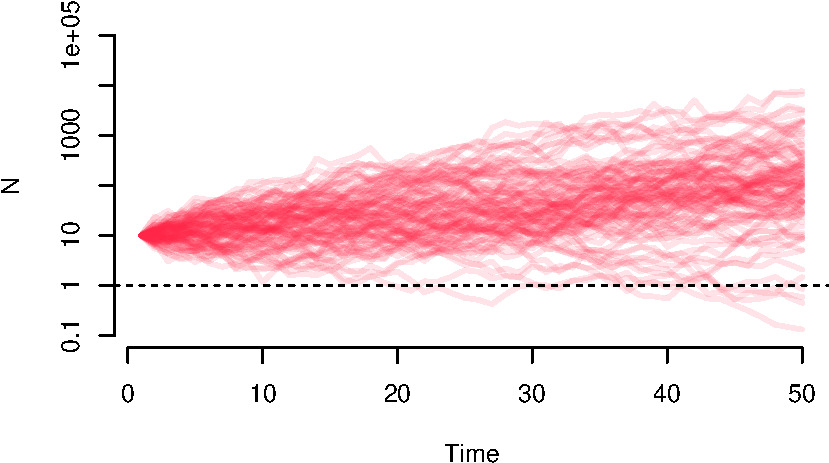
\includegraphics{BB512_files/figure-latex/stochProjection-1} 

}

\caption{An example of stochastic population projection (100 simulations for 50 generations)}\label{fig:stochProjection}
\end{figure}

\hypertarget{basic-logistic-population-growth}{%
\chapter{Basic logistic population
growth}\label{basic-logistic-population-growth}}

Population sizes have upper limits -- they can only get so large. This
is often modeled with the `logistic growth' model\footnote{This is
  equation 2.4 in Gotelli}:

\(N_{t+1}=N_{t}+r_{d} N_{t}\left(1-\frac{N_{t}}{K}\right)\)

This equation models population at time \(t+1\) (\(N_{t+1}\)) as a
function of the population at time \(t\) (\(N_t\)), the \emph{discrete
growth factor} (\(r_d\)), and carrying capacity of the environment
(\(K\)).

The idea is that the growth rate of the population (the difference
between \(N_{t+1}\) and \(N_t\)) decreases as the population increases
in size. When the population size at \(N_t\) is equal to the
\emph{carrying capacity} of the environment (\(K\)), the population
growth rate is zero. For example, if the carrying capacity of the
population is \emph{200}, and there are already \emph{200} individuals
in the population, then the size of the population will remain unchanged
through time (\(N_{t+1} = N_t = 200\)).

The aim of this Excel-based exercise is to explore this model and help
you get an intuitive understanding of it by looking at it from different
perspectives. Even though it is a fairly simple model, it leads us to
some useful biological insights.

Download and open the Excel file:
\href{https://www.dropbox.com/s/oxxyyn4zf4wsvkg/Basic\%20Logistic\%20Growth.xlsx?dl=1}{\texttt{Basic\ Logistic\ Growth.xslx}}.

You will see that there are three blocks of numbers, and three graphs.
During the exercise you only need to edit the pink block.

The pink block gives the important parameters of the logistic model:

\begin{itemize}
\tightlist
\item
  \texttt{Initial\ N} = the starting population size at time 1.
\item
  \texttt{r\_d} = the maximum per capita population growth rate
  (\(r_d\)). When \(r_d\) is 0, the population does not grow. When
  \(r_d\) is \(>\) 0 the population grows, and when it is \(<\) 0 it
  declines. The population cannot fall below 0.
\item
  \texttt{K} = the carrying capacity of the population.
\end{itemize}

The initial values for these are \emph{10}, \emph{0.8} and \emph{200}
respectively.

In this exercises you will be altering these parameters and observing
the outcome in the 3 graphs which show:

\begin{enumerate}
\def\labelenumi{\arabic{enumi}.}
\tightlist
\item
  The population size through time.
\item
  The per capita growth rate of the population in relation to population
  size
\item
  The relationship between population size at time t and at time t+1
\end{enumerate}

\hypertarget{graph-1}{%
\section{Graph 1}\label{graph-1}}

First -- take a look at \textbf{Graph 1}.

\begin{itemize}
\tightlist
\item
  What is the maximum population size?
\item
  How does this compare to carrying capacity (\texttt{K})?
\item
  What do you predict to happen if you increase \texttt{K} to
  \emph{300}? (try it)
\end{itemize}

\begin{itemize}
\tightlist
\item
  At what time do you reach the maximum population size?
\item
  If you halved the discrete growth factor (\texttt{r\_d}) to
  \emph{0.4}, what do you think will happen to the dynamics this time?
  (try it)
\end{itemize}

\begin{itemize}
\tightlist
\item
  What do you think will happen if you \texttt{r\_d} to \emph{1.8}? (try
  it)
\item
  What do you notice about the population size through time?
\item
  How does the maximum population size compare with the carrying
  capacity? How would you describe the `\emph{dynamics}' of this
  population?
\end{itemize}

\begin{itemize}
\tightlist
\item
  What happens if you increase the \texttt{r\_d} even more, to \emph{2}
  or \emph{2.1}?
\item
  And even more to \emph{2.8}, \emph{2.9} or \emph{3}?
\item
  How would you describe these dynamics?
\item
  Is there a limit to how high \texttt{r\_d} can be? (hint: populations
  go extinct if N \(<\) 0).
\end{itemize}

Finally, compare the population trajectory in \textbf{Graph 1} for
populations with \texttt{r\_d}= \emph{2.8} and \emph{2.81}. Then compare
the trajectories where you fix \texttt{r\_d} at \emph{2.8} but vary
initial population size by a small amount (e.g.~\emph{1}). Imagine you
were a population manager -- would these populations be easy or hard to
predict? What kinds of species have high population growth rates like
these?

\hypertarget{graphs-2-3}{%
\section{Graphs 2 \& 3}\label{graphs-2-3}}

Now let's turn to \textbf{Graphs 2} and \textbf{3}.

In \textbf{Graph 2}, notice that the per capita growth rate always
declines linearly with population size (\texttt{N}). Where does it cross
the x-axis line? Modify the carrying capacity (\texttt{K}) -- what do
you notice?

\textbf{Graph 3} is shaped like a parabola, starting with small values,
increasing to a maximum, then declining to small values again. The
position of the maximum is dependent on the values of \texttt{K} and
\texttt{r\_d}. When \texttt{r\_d} is small (around \emph{1}), the peak
is at \(x = K\) and \(y = K\). Explore (1) how the peak moves around if
you fix one of \texttt{K} or \texttt{r\_d} and alter the other parameter
and (2) how the slope of the line changes at \(N_t = K\).

\emph{Hint: the slope of the line changes from positive to negative as
\texttt{r\_d} increases.}

\begin{do-something}
These three graphs are simply different ways to visualize the same
model. It is important that you can make the connections between these
graphs.

How would the same plots look for regular exponential growth?
\end{do-something}

Some useful keywords:

\begin{itemize}
\tightlist
\item
  Oscillation
\item
  Cycle/cyclic dynamics
\item
  Stable-limit cycle (2-point, 3-point limit cycle)
\item
  Chaos/Chaotic dynamics
\item
  Unpredictable/predictable
\end{itemize}

\hypertarget{deeper-into-logistic-growth}{%
\chapter{Deeper into logistic
growth}\label{deeper-into-logistic-growth}}

The purpose of this exercise is (i) to look at the relationships between
the exponential (or geometric) growth model and the logistic growth
model and (ii) to emphasise different ways of looking at the models.

I will begin by showing the equations on the blackboard/whiteboard for
exponential and logistic growth. I will highlight how the logistic model
is a simple extension of the exponential model. I will show that when K
is infinite the model \(\frac{d N}{d t}=r N\left(1-\frac{N}{K}\right)\),
simplifies to the exponential model (\(\frac{d N}{d t}=r N\)), because
the \((1-\frac{N}{K})\) bit drops out of the equation.\footnote{These
  are equations 2.1 and 1.1 in Gotelli.}

The same is true for the discrete version of the logistic growth model:
Compare the equation
\(N_{t+1}=N_{t}+r_{d} N_{t}\left(1-\frac{N_{t}}{K}\right)\) with
\(N_{t+1}=N_{t}+r_{d} N_{t}\).\footnote{These are Expression 1.13 (page.
  11) and equation 2.4 from Gotelli.}

You can then look at the Excel file
\href{https://www.dropbox.com/s/4xq399z7skl1akv/Deeper\%20into\%20Logistic\%20Growth.xlsx?dl=1}{\texttt{Deeper\ Into\ Logistic\ Growth.xlsx}}.

\hypertarget{different-views-of-the-basic-logistic-growth-model}{%
\section{Different views of the basic logistic growth
model}\label{different-views-of-the-basic-logistic-growth-model}}

Take a look at the \texttt{BasicLogistic} Excel worksheet/ark.

Focus first on \textbf{Figure 1}.

Enter different values for \texttt{r\_d}, e.g.~0.8, 1.2, 1.8, 2.4,
2.7\ldots{}

Can you describe the dynamics of the population time series in Figure 1
using some of the following vocabulary: Oscillation, damped oscillation,
stable cycle, 2-point cycle, chaotic, unpredictable, predictable?

Now focus on \textbf{Figure 2}.

This figure shows the per capita population growth rate as a function of
population size at time \(t\). Note where the line intercepts the x- and
y-axes.

What do you notice about these values? Hint: what are the values you
have set for \texttt{r\_d} and \texttt{K}? Try varying those values.

On paper, make a sketch of a graph for per capita population growth rate
as a function of population size at time t for a logistic model with
\(r_d\) = 1.5 and \(K\) = 250, indicating the values of the intercepts.
Check your sketch by entering those values into the Excel model.

Based on what you know about what happens to the population dynamics for
different values of \(r_d\) and what you have just seen in Figure 2, you
should now be able to sketch fairly accurate cartoon graphs if you are
given values for \(r_d\) and \(K\)!

\emph{Without using Excel}, draw a population time series, and a graph
of per capita growth rate vs.~N for when initial population size is 10,
\(r_d\) is 1.9 and \(K\) is 500. Check your graph using Excel.

Focus now on \textbf{Figure 3}.

Population growth rate is \(dN/dt\) - the rate of change in \(N\)
(\(dN\), change in population size) per unit time (\(dt\)). You should
now explore how \emph{Figure 3} relates to the values used in the
equation by changing the \(r_d\) and \(K\) values and looking at
\emph{Figure 3}.

Can you see how \emph{Figures 1}, \emph{2} and \emph{3} are connected?

At what population sizes is the population growth rate 0 (\(dN/dt\))?
What is the population size at which the population growth is rate
maximized?

Now lets look back on \textbf{Exponential growth}.

How do the relationships in Figures 1, 2 and 3, differ from the
equivalent figures for logistic growth. Try to draw graphs of Figures 1,
2 and 3 for the exponential growth model.

\begin{itemize}
\tightlist
\item
  Fig 1. Population size (\(N\)) through time (\(t\)).
\item
  Fig 2. Per capita growth rate (\(\frac{1}{N} \frac{dN}{dt}\))
  vs.~population size (\(N\))
\item
  Fig 3. Population growth rate (\(\frac{dN}{dt}\)) vs.~population size
  (\(N\)) (see figure 2.4 in Gotelli)
\end{itemize}

\hypertarget{adding-a-time-lag}{%
\section{Adding a time lag}\label{adding-a-time-lag}}

This relates to \emph{Equation 2.3} in Gotelli (and pages 32-35).

\(\frac{d N}{d t}=r N\left(1-\frac{N_{t-\tau}}{K}\right)\)

Look at the Excel Worksheet/Ark called \texttt{TimeLag}.

Adding a time lag to logistic model can complicate the dynamics (by
introducing cycling). The 3rd Excel tab has an exercise showing that if
you add in a time lag to the logistic function it modifies the dynamics.
The purpose of this Excel sheet is to allow you to prove this to
yourself!

You will need to carefully modify the Excel formula so that instead of
referring back to the population size at \(N_{t-1}\), it refers back to
\(N_{t-1}\) etc. Remember to drag the formula down to all the other
years (or use the shortcut I will show you).

Start with a small \(r_d\) that gives a smooth convergence to K with an
ordinary logistic model. Add in a 1-year time lag and show that this
generates cyclic dynamics. This shows that this simple ``quirk of life
history'' (a time lag) can generate cycling, even if the population
growth rate is low.

\hypertarget{optional-cobweb-diagrams}{%
\section{Optional: Cobweb diagrams}\label{optional-cobweb-diagrams}}

The cobweb diagram is another useful tool to visualize and explore
dynamics of logistic models. See the book section by Mathiopoulos on
itsLearning. They would be very hard to implement in Excel, so I have
made a webapp: (\url{https://jonesor.shinyapps.io/cobweb/})

The graph shows a ``track'' which follows the fate of a population. The
track bounces between the parabola describing the relationship between
\(N_t\) and \(N_{t+1}\) (Figure 3.1 in the excel sheet) and a 1:1 line.
Try altering \(r_d\) in the model and observe what different types of
dynamics look like with this ``view.'' Check out what happens if you
modify the starting population size. You should see that for non-chaotic
dynamics, the starting population size doesn't affect the fate of the
population. For example, set initial population to be 0.01, and \(r_d\)
to be 0.9. You should see damped oscillations. Now move the initial
population slider. You should see that the population always ends up
with the same dynamics, heading towards carrying capacity.

\hypertarget{life-tables-and-survivorship-types}{%
\chapter{Life tables and survivorship
types}\label{life-tables-and-survivorship-types}}

Life tables are tables that shows for each age, the probability that an
individual of that age will die before the next birthday
(\emph{probability of death}). This exercise deals with so-called
\textbf{cohort life tables} which, as the name implies, follows a
``\emph{cohort}'' of individuals from birth until they all die. A cohort
is the group of individuals born within a particular time interval
(e.g.~``\emph{all individuals born in 1998}'').

Life tables have been used extensively in population biology, in human
demography and in epidemiology. They are also important outside of
biology, e.g.~in the management of product life-cycles, such as in cars
or other machinery.

The basic algebra used in life tables is explained in Gotelli Chapter 3
(see table 3.1 for an example).

The purpose of this exercise is:

\begin{enumerate}
\def\labelenumi{\arabic{enumi}.}
\tightlist
\item
  to allow you to calculate a life table yourself in Excel;
\item
  to develop your Excel modeling skills by asking you to make the
  calculations following the equations given in Gotelli (and in the
  lecture slides);
\item
  to allow you to explore different types of survivorship (Type I, II
  and III) and consider the relationship between these life tables and
  ``life history strategy'' (more on this in the evolution part of the
  course).
\end{enumerate}

Open the Excel file
\texttt{{[}Life\ tables\ exercises.xlsx{]}(https://www.dropbox.com/s/ox0rk05zdwzrmwy/Life\%20tables\%20exercises.xlsx?dl=1)}.

The file has three worksheets (``\emph{Life table},''
``\emph{Survivorship Curves}'' and ``\emph{Gotelli Table 3.1 example}.''

Let's start with ``\textbf{Life table}.''

The aim now is to use Excel as a modeling tool to produce a life table.
I have provided some initial data collected from a cohort of animals. I
know how many individuals survive each year (how many ``enter the
interval''). I also know how many babies (on average) are produced by
each female.

Start by calculating survivorship (\(l_x\)). Survivorship is the
\textbf{probability of survival to a particular age}. Therefore, at time
0, \(l_0 = 1\), since everyone is alive at this point. The next value
(\(l_1\)) must be calculated based on the number alive at that point. In
this case it is \(352/500 = 0.704\). You must generalize this
calculation into a formula that can be dragged to fill column \texttt{D}
in the worksheet. In algebraic form, the equation is \(l_x = S_x/S_0\).

Next, you can calculate age specific \textbf{survival probability}. Note
that this is different from lx. Survival probability is simply the
probability that an individual will survive its current age class.
i.e.~what is the probability that an individual currently aged 2 will
survive to become age 3. In this case, the \(254/298 = 0.852\). The
calculation is \(g_x = l_{x-1}/l_x\), or \(S_{x-1}/S_x\).

Now complete the remaining two columns, and use them to calculate (a)
\(R_0\); (b) \textbf{Generation time}; and an approximation of \(r\).
\textbf{Tip} You need to understand the use of the \texttt{\$} symbol in
Excel, and how to drag the selected area to place the formula in the
column. Refer to the sheet ``\emph{Gotelli Table 3.1 example}'' if you
get stuck (you should be able to see the formulae used there.

In the second part we focus on the \textbf{Survivorship Curves}
worksheet. The aim here is to start to explore how different types of
organisms with different ways of life (``\textbf{life history
strategies}'') can have qualitatively different kinds of life tables.
The most important thing to observe is the difference in
\textbf{survivorship curves} (\(l_x\)). These changes become very
obvious when you plot the log-transformed survivorship against age.

In the Excel worksheet, I have placed tables showing the fate of cohorts
of three populations of different species. Your job now is to calculate
the survivorship curve (\(l_x\)) for these species, take the natural log
(using formula \texttt{=log(C3)}, for the first population,
\texttt{=log(H3)} for the second population etc.

You should see that the graphs automatically fill up with lines. These
show Type I, II and III survivorship.

\hypertarget{matrix-population-modelling}{%
\chapter{Matrix population
modelling}\label{matrix-population-modelling}}

Think of an organism you would like to model the dynamics of. It could
be a mammal, a bird, a fish, insect or tree \ldots{} real or fantasy.

Think about their life cycle, and draw it as a life cycle diagram with
circles indicating the stages and arrows representing transitions
between stages and reproduction. Next to the arrows, write values for
survival probability and fecundity (number of babies) using your
biological knowledge.

Things to think about:

\begin{itemize}
\tightlist
\item
  Is it age based or stage based?
\item
  How many stages are there?
\item
  If it is stage, how are stages defined? E.g. by size, by development,
  etc.
\item
  Are the survival and fecundity higher in earlier or later life?
\item
  Does the organism skip stages?
\item
  Does the organism move backwards through the life cycle?
\end{itemize}


\includegraphics[width=0.3\linewidth]{BB512_files/figure-latex/unnamed-chunk-30-1}

Turn this diagram into a matrix population model by filling in a square
of survival/fecundity values. There is space below for up to a 4-stage
matrix model.


\includegraphics{BB512_files/figure-latex/unnamed-chunk-31-1.pdf}

Working with matrices is very tedious in Excel. However, in R you can
use this information to predict the future dynamics of the population,
and estimate population growth rate, and generation time etc.

Open up \textbf{RStudio}, and lets see if we can predict future
dynamics. First you will need to install a package called
\texttt{popdemo}.

\begin{Shaded}
\begin{Highlighting}[]
\FunctionTok{install.packages}\NormalTok{(}\StringTok{"popdemo"}\NormalTok{)}
\end{Highlighting}
\end{Shaded}

You only need to install packages once. After thatyou can load the
package for use by using the \texttt{library} function.

\begin{Shaded}
\begin{Highlighting}[]
\FunctionTok{library}\NormalTok{(popdemo)}
\end{Highlighting}
\end{Shaded}

You can put your matrix into R like in the example below (change the
numbers to match YOUR model). If your model has fewer, or more, stages
then you will need to modify the code a bit. Ask for help if you get
stuck.

\begin{Shaded}
\begin{Highlighting}[]
\NormalTok{    A }\OtherTok{\textless{}{-}} \FunctionTok{matrix}\NormalTok{(}\FunctionTok{c}\NormalTok{( }\FloatTok{0.00}\NormalTok{, }\FloatTok{0.00}\NormalTok{, }\FloatTok{4.00}\NormalTok{, }\FloatTok{2.00}\NormalTok{,}
                   \FloatTok{0.10}\NormalTok{, }\FloatTok{0.00}\NormalTok{, }\FloatTok{0.00}\NormalTok{, }\FloatTok{0.00}\NormalTok{,}
                   \FloatTok{0.50}\NormalTok{, }\FloatTok{0.20}\NormalTok{, }\FloatTok{0.00}\NormalTok{, }\FloatTok{0.00}\NormalTok{,}
                   \FloatTok{0.00}\NormalTok{, }\FloatTok{0.30}\NormalTok{, }\FloatTok{0.40}\NormalTok{, }\FloatTok{0.30}\NormalTok{),}
                \AttributeTok{byrow =} \ConstantTok{TRUE}\NormalTok{, }\AttributeTok{nrow =} \DecValTok{4}\NormalTok{)}
\end{Highlighting}
\end{Shaded}

And now you can use the project function to project what happens to the
population, then plot it. Look at what happens if you log or don't log
the y-axis. First you need to define an initial starting population
structure.

In my example, I have 4 stages, so I have 4 values for the initial
population sizes. Then I use the \texttt{popdemo} function
\texttt{project} to do a population projection for 10 time steps.

\begin{Shaded}
\begin{Highlighting}[]
\NormalTok{initial }\OtherTok{\textless{}{-}} \FunctionTok{c}\NormalTok{(}\DecValTok{10}\NormalTok{,}\DecValTok{5}\NormalTok{,}\DecValTok{3}\NormalTok{,}\DecValTok{3}\NormalTok{)}
\NormalTok{pr }\OtherTok{\textless{}{-}}\NormalTok{ popdemo}\SpecialCharTok{::}\FunctionTok{project}\NormalTok{(A, }\AttributeTok{vector =}\NormalTok{ initial, }\AttributeTok{time=}\DecValTok{10}\NormalTok{)}
\end{Highlighting}
\end{Shaded}

Take a look at \texttt{pr}, the projected population. This gives you the
total population size, and below that the population sizes in each
stage.

\begin{Shaded}
\begin{Highlighting}[]
\NormalTok{pr}
\end{Highlighting}
\end{Shaded}

\begin{verbatim}
## 1 deterministic population projection over 10 time intervals.
## 
##  [1]   21.0000   28.6000   45.9800   68.7940  110.7142  167.8147  267.2773
##  [8]  408.6193  646.1858  993.7152 1563.8309
\end{verbatim}

You can access the population sizes of the different stages using
\texttt{vec(pr)}.

\begin{Shaded}
\begin{Highlighting}[]
\FunctionTok{vec}\NormalTok{(pr)}
\end{Highlighting}
\end{Shaded}

\begin{verbatim}
##              S1       S2        S3        S4
##  [1,]   10.0000  5.00000   3.00000   3.00000
##  [2,]   18.0000  1.00000   6.00000   3.60000
##  [3,]   31.2000  1.80000   9.20000   3.78000
##  [4,]   44.3600  3.12000  15.96000   5.35400
##  [5,]   74.5480  4.43600  22.80400   8.92620
##  [6,]  109.0684  7.45480  38.16120  13.13026
##  [7,]  178.9053 10.90684  56.02516  21.44000
##  [8,]  266.9806 17.89053  91.63403  32.11412
##  [9,]  430.7643 26.69806 137.06842  51.65501
## [10,]  651.5837 43.07643 220.72178  78.33329
## [11,] 1039.5537 65.15837 334.40714 124.71163
\end{verbatim}

Let's plot this\ldots{}

\begin{Shaded}
\begin{Highlighting}[]
\NormalTok{pop }\OtherTok{\textless{}{-}} \FunctionTok{vec}\NormalTok{(pr)}
\FunctionTok{matplot}\NormalTok{(pop,}\AttributeTok{type=}\StringTok{"l"}\NormalTok{,}\AttributeTok{log=}\StringTok{"y"}\NormalTok{)}
\FunctionTok{legend}\NormalTok{(}\StringTok{"topleft"}\NormalTok{,}\AttributeTok{legend =} \FunctionTok{colnames}\NormalTok{(pop),}\AttributeTok{col=}\DecValTok{1}\SpecialCharTok{:}\FunctionTok{ncol}\NormalTok{(pop),}\AttributeTok{lty=}\DecValTok{1}\SpecialCharTok{:}\FunctionTok{ncol}\NormalTok{(pop))}
\end{Highlighting}
\end{Shaded}

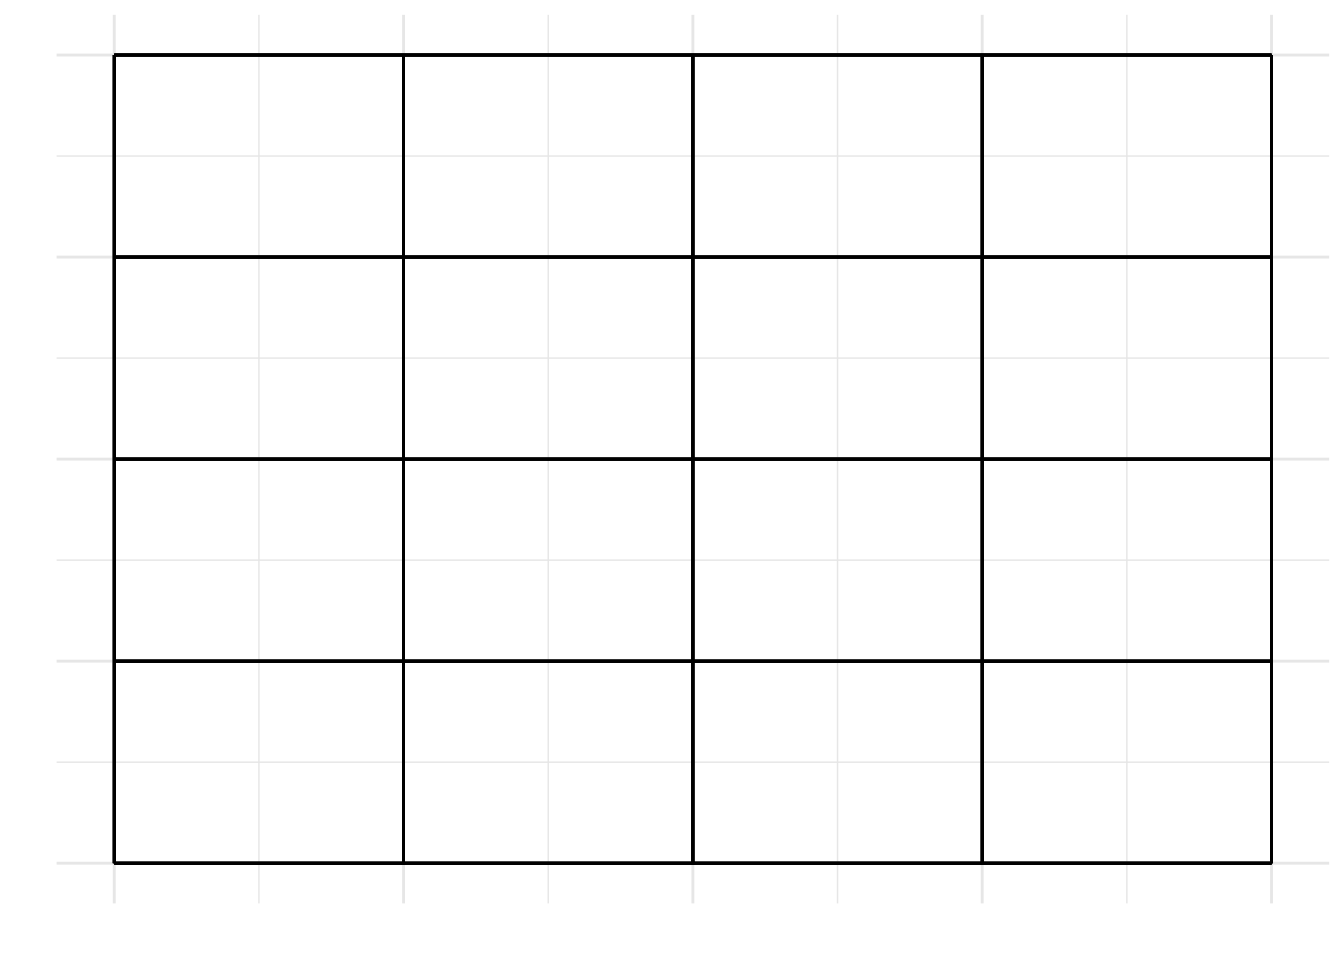
\includegraphics{BB512_files/figure-latex/unnamed-chunk-38-1.pdf}

You should see that the population increases exponentially. The
population growth rate is the so-called ``\emph{dominant eigenvalue}''
of the matrix \textbf{A}.

We can ask R for the \emph{eigen values} and \emph{eigen vectors}. These
are the population growth rate (\(\lambda\)) and the stable stage
distribution (\emph{SSD}) and the reproductive values (\emph{RV}) of the
different stages. \emph{SSD} is the expected \emph{proportion} of
individuals in the different stage classes at equilibrium and \emph{RV}
is the expected number of future offspring by individuals in each stage.

You can see that in this case, using my example values the population is
growing 55.74\% per year.

\begin{Shaded}
\begin{Highlighting}[]
\FunctionTok{eigs}\NormalTok{(A)}
\end{Highlighting}
\end{Shaded}

\begin{verbatim}
## $lambda
## [1] 1.557365
## 
## $ss
## [1] 0.66068003 0.04242295 0.21756281 0.07933420
## 
## $rv
## [1] 0.6831674 0.4705100 2.0337794 1.0866656
\end{verbatim}

\hypertarget{your-turn}{%
\section{Your turn\ldots{}}\label{your-turn}}

\begin{enumerate}
\def\labelenumi{\arabic{enumi})}
\tightlist
\item
  by editing the inputs in the code above, make a projection for
  \textbf{your} data.
\item
  plot the results (using the R code here)
\item
  what is the health of your population?
\end{enumerate}

\hypertarget{an-evolutionary-experiment}{%
\section{An evolutionary experiment}\label{an-evolutionary-experiment}}

You can think of lambda (population growth rate) as being a measure of
fitness. Imagine that some of your population had a mutation that caused
them to have, say, 1 extra baby, but at the expense of reduced survival
in one of the younger stages. Would this mutation persist in the
population?

\hypertarget{lotka-volterra-competition}{%
\chapter{Lotka-Volterra competition}\label{lotka-volterra-competition}}

In ecology the there is a ``rule'' called the ``competitive exclusion
principle'' which states that two species cannot coexist unless their
niches are sufficiently different.

How different do their niches need to be for coexistence? The general
idea is that coexistence can occur if each species limits its own
population growth rate more than it limits the growth rate of the other
species.

If there the niches overlap too much, one species will competitively
exclude the other (i.e.~forces the other to extinction).

In this class you will be working from a PDF available
\href{https://www.dropbox.com/s/oukr39oq0rsn8il/9.\%20Interspecific\%20Competition\%20and\%20Competitive\%20Exclusion.pdf?dl=1}{here}
to explore this idea.

This PDF walks you through the creation of an Excel spreadsheet
exploring interspecific competition and competitive exclusion using the
Lotka-Volterra model.

Your task:

\begin{itemize}
\tightlist
\item
  Create the Excel spreadsheet by following the instructions in the PDF
\item
  Use the Lotka-Volterra model you have created to answer the questions
  at the end of the PDF.
\end{itemize}

\hypertarget{the-questions}{%
\subsection{The questions}\label{the-questions}}

\begin{enumerate}
\def\labelenumi{\arabic{enumi}.}
\tightlist
\item
  What parameter values will cause species 1 to exclude species 2 from
  the habitat? What do these values mean in ecological terms?
\item
  What parameter values will reverse this outcome? What do these values
  mean in ecological terms?
\item
  What parameter values will allow the two species to coexist
  indefinitely and stably? What do these values mean in ecological
  terms?
\item
  Are there parameter values under which the outcome depends on initial
  population sizes or rates of population growth? What do these values
  mean in ecological terms?
\end{enumerate}

\hypertarget{lotka-volterra-predator-prey-dynamics}{%
\chapter{Lotka-Volterra predator-prey
dynamics}\label{lotka-volterra-predator-prey-dynamics}}

In the classic Lotka-Volterra predator-prey model (Rosenzweig and
MacArthur 1963), the predator and prey populations grow exponentially.
Modifications to the model include the availability of refuges (places
where the prey are safe from predators) and carrying capacity
(i.e.~using logistic growth).

In this class you will follow a PDF worksheet
(\href{https://www.dropbox.com/s/bhwoe161wp9p6hp/10.\%20Predator-prey\%20dynamics.pdf?dl=1}{here})
which guides you to build and explore a Lotka-Volterra predator-prey
model in Excel. The model has parameters for the prey and for the
predator, and you will explore how these parameters influence the
dynamics of the populations.

The worksheet is divided into three parts. We will mainly \textbf{focus
on Part 1} - the basic model - in the class.

Part 2 modifies the basic model to include a refuge, and part 3 modifies
the model to include carrying capacity. Feel free to continue to work on
these if there is time, and if you are interested.

\hypertarget{reference}{%
\subsection{Reference}\label{reference}}

Rosenzweig, M. L. and R. H. MacArthur. 1963. Graphical representation
and stability conditions of predator-prey interactions. \emph{American
Naturalist} 97: 209--223.

\hypertarget{part-evolution}{%
\chapter*{(PART) Evolution}\label{part-evolution}}
\addcontentsline{toc}{chapter}{(PART) Evolution}

\hypertarget{from-population-biology-to-fitness}{%
\chapter{From population biology to
fitness}\label{from-population-biology-to-fitness}}

The purpose of this practical is to draw clear links between the first
part of the course (population biology) and the second part of the
course (evolution).

We will focus on the concept of \textbf{fitness}.

Fitness is a slippery concept, but it is widely accepted that it is
closely related to population growth rate. In this class you will
explore this concept using some mathematical modelling (aagh!).

\begin{do-something}
This practical uses RStudio (R). It is similar to the previous exercise
on matrix population models, but ask for help if you get stuck!
\end{do-something}

\hypertarget{an-in-silico-experiment}{%
\section{\texorpdfstring{An \emph{in silico}
experiment}{An in silico experiment}}\label{an-in-silico-experiment}}

As you learned in the classes on age and stage structured population
dynamics differences in survival and reproduction can be modelled using
matrix population models (MPMs). These models can be simple or complex,
and can be thought of as mathematical descriptions of the life history
of the species (or population) in a particular environment.

In an earlier you will have played with construction and analyses of
these models by creating MPMs for species with different life histories
such as high juvenile survival, or low juvenile survival etc.

We will first need to load the \texttt{popdemo} package like this. Note
that if you have not installed this package you should first install it
with the command \texttt{install.packages("popdemo")}.

\begin{Shaded}
\begin{Highlighting}[]
\FunctionTok{library}\NormalTok{(popdemo)}
\end{Highlighting}
\end{Shaded}

Let's set up our baseline model. This model describes a population of
some mammal species which we have divided into 3 stages: juvenile, adult
and senescent (old).

\begin{Shaded}
\begin{Highlighting}[]
\NormalTok{A1 }\OtherTok{\textless{}{-}} \FunctionTok{matrix}\NormalTok{(}\FunctionTok{c}\NormalTok{(}\FloatTok{0.00}\NormalTok{, }\FloatTok{4.00}\NormalTok{, }\FloatTok{2.00}\NormalTok{, }
               \FloatTok{0.10}\NormalTok{, }\FloatTok{0.80}\NormalTok{, }\FloatTok{0.00}\NormalTok{, }
               \FloatTok{0.00}\NormalTok{, }\FloatTok{0.10}\NormalTok{, }\FloatTok{0.40}\NormalTok{), }
            \AttributeTok{byrow =} \ConstantTok{TRUE}\NormalTok{, }\AttributeTok{nrow =} \DecValTok{3}\NormalTok{)}
\end{Highlighting}
\end{Shaded}

You can ``read'' the matrix by looking at the columns and rows: a value
in the column \textbf{3} and row \textbf{1} tells you the ``transition''
\textbf{from} stage 3 \textbf{to} stage 1. In this case, it is saying
that an individual in the adult age class produces an average of 5
babies, and one from the senescent age class produces 1 baby. Juveniles
have a probability of 0.1 (10\% chance) to survive to adulthood (and
they reach maturity in 1 year, so there is no ``stasis'' where they can
remain being juveniles). Adults can survive in 2 ways, they can survive
and remain as adults (probability = 0.8) or they can survive and
transition to being in the sensescent age class (probability = 0.1).
Therefore, the total survival probability is 0.9. Senescent adults
survive less well (probability = 0.4).

We can project a population like this:

\begin{Shaded}
\begin{Highlighting}[]
\NormalTok{initial }\OtherTok{\textless{}{-}} \FunctionTok{c}\NormalTok{(}\DecValTok{10}\NormalTok{,}\DecValTok{5}\NormalTok{,}\DecValTok{3}\NormalTok{) }\CommentTok{\# just some random numbers}
\NormalTok{pr }\OtherTok{\textless{}{-}}\NormalTok{ popdemo}\SpecialCharTok{::}\FunctionTok{project}\NormalTok{(A1, }\AttributeTok{vector =}\NormalTok{ initial, }\AttributeTok{time=}\DecValTok{8}\NormalTok{)}
\end{Highlighting}
\end{Shaded}

Take a look at \texttt{pr}, the projected population. This gives you the
total population size, and below that the population sizes in each
stage.

\begin{Shaded}
\begin{Highlighting}[]
\NormalTok{pr}
\end{Highlighting}
\end{Shaded}

\begin{verbatim}
## 1 deterministic population projection over 8 time intervals.
## 
## [1] 18.00000 32.70000 31.18000 37.51200 42.93080 50.15272 58.36605 68.04116
## [9] 79.29730
\end{verbatim}

You can access the population sizes of the different stages using
\texttt{vec(pr)}.

\begin{Shaded}
\begin{Highlighting}[]
\FunctionTok{vec}\NormalTok{(pr)}
\end{Highlighting}
\end{Shaded}

\begin{verbatim}
##             S1       S2       S3
##  [1,] 10.00000  5.00000 3.000000
##  [2,] 26.00000  5.00000 1.700000
##  [3,] 23.40000  6.60000 1.180000
##  [4,] 28.76000  7.62000 1.132000
##  [5,] 32.74400  8.97200 1.214800
##  [6,] 38.31760 10.45200 1.383120
##  [7,] 44.57424 12.19336 1.598448
##  [8,] 51.97034 14.21211 1.858715
##  [9,] 60.56588 16.56672 2.164697
\end{verbatim}

Let's plot this\ldots{} Check out how, after a ``transient'' period,
there is exponential growth in all stages of the population. The
population is growing steadily with a fixed population growth rate
(\(\lambda\)).

\begin{Shaded}
\begin{Highlighting}[]
\NormalTok{pop }\OtherTok{\textless{}{-}} \FunctionTok{vec}\NormalTok{(pr)}
\FunctionTok{matplot}\NormalTok{(pop,}\AttributeTok{type=}\StringTok{"l"}\NormalTok{,}\AttributeTok{log=}\StringTok{"y"}\NormalTok{)}
\FunctionTok{legend}\NormalTok{(}\StringTok{"topleft"}\NormalTok{,}\AttributeTok{legend =} \FunctionTok{colnames}\NormalTok{(pop),}\AttributeTok{col=}\DecValTok{1}\SpecialCharTok{:}\FunctionTok{ncol}\NormalTok{(pop),}\AttributeTok{lty=}\DecValTok{1}\SpecialCharTok{:}\FunctionTok{ncol}\NormalTok{(pop))}
\end{Highlighting}
\end{Shaded}

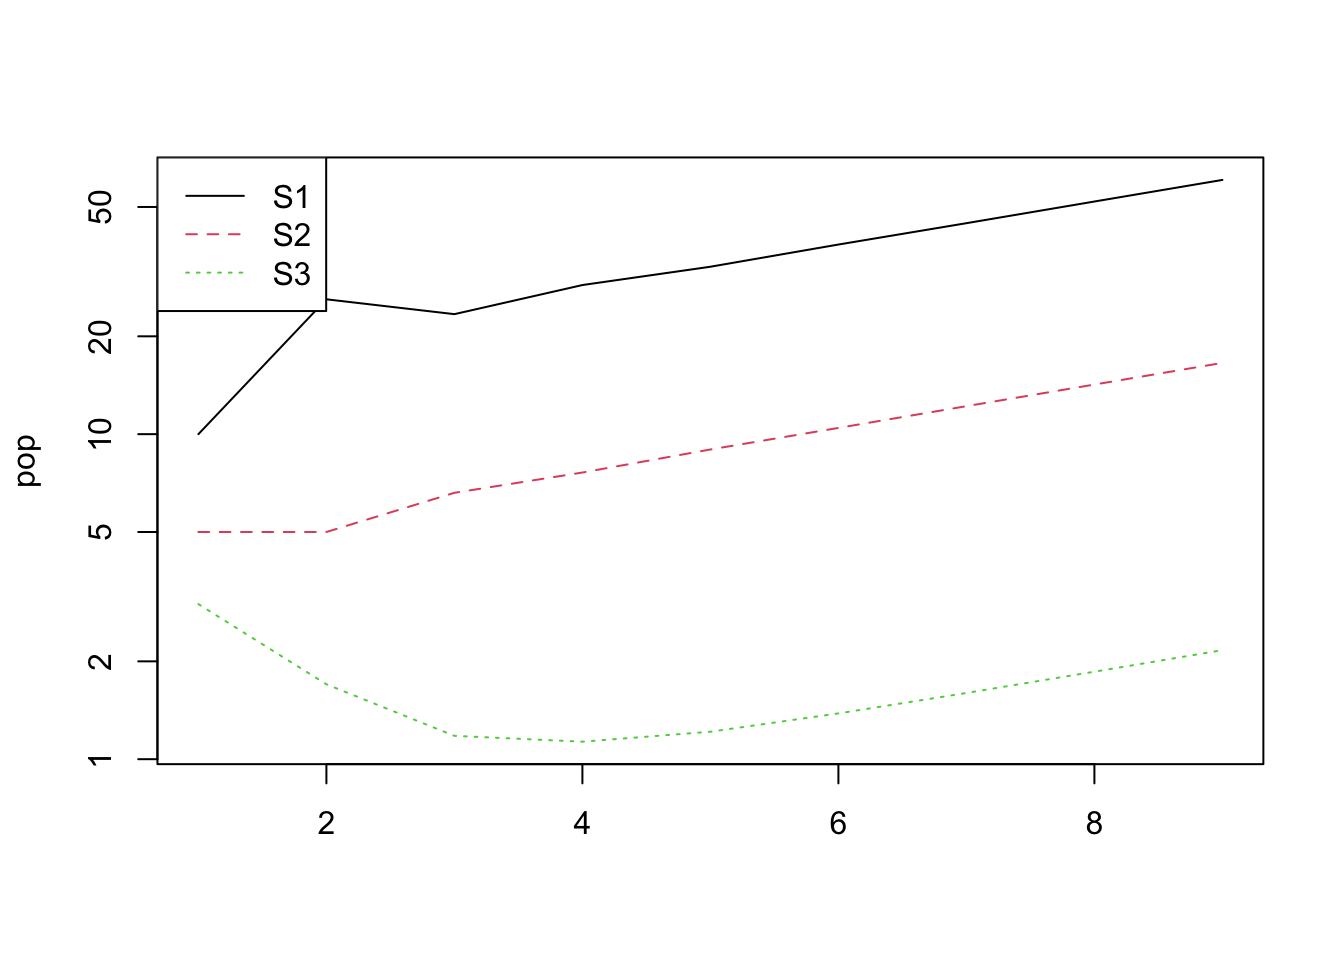
\includegraphics{BB512_files/figure-latex/unnamed-chunk-50-1.pdf}

You can see that the population is increasing and we can calculate the
precise population growth rate (\(\lambda\)) like this:

\begin{Shaded}
\begin{Highlighting}[]
\FunctionTok{eigs}\NormalTok{(A1)}\SpecialCharTok{$}\NormalTok{lambda}
\end{Highlighting}
\end{Shaded}

\begin{verbatim}
## [1] 1.165587
\end{verbatim}

Thus, the population is growing at 16.56\% per year.

So where does evolution come in?

\hypertarget{the-link-to-fitness}{%
\section{The link to fitness}\label{the-link-to-fitness}}

In this population consider that suddenly a mutation arises in an
individual parent that causes it to give more care to their offspring.
For example, maybe they provide milk with a higher fat content, or build
a safer nest. Whatever the mechanism, let's assume that it results in a
small increase in juvenile survival.

We can simulate this by increasing the juvenile survival in the matrix
model from 0.10 to 0.11.

\begin{Shaded}
\begin{Highlighting}[]
\NormalTok{A2 }\OtherTok{\textless{}{-}} \FunctionTok{matrix}\NormalTok{(}\FunctionTok{c}\NormalTok{(}\FloatTok{0.00}\NormalTok{, }\FloatTok{4.00}\NormalTok{, }\FloatTok{2.00}\NormalTok{, }
               \FloatTok{0.11}\NormalTok{, }\FloatTok{0.80}\NormalTok{, }\FloatTok{0.00}\NormalTok{, }
               \FloatTok{0.00}\NormalTok{, }\FloatTok{0.10}\NormalTok{, }\FloatTok{0.40}\NormalTok{), }
            \AttributeTok{byrow =} \ConstantTok{TRUE}\NormalTok{, }\AttributeTok{nrow =} \DecValTok{3}\NormalTok{)}
\end{Highlighting}
\end{Shaded}

What effect does that have on population growth rate?

\begin{Shaded}
\begin{Highlighting}[]
\FunctionTok{eigs}\NormalTok{(A2)}\SpecialCharTok{$}\NormalTok{lambda}
\end{Highlighting}
\end{Shaded}

\begin{verbatim}
## [1] 1.192317
\end{verbatim}

The small increase in juvenile survival has resulted in a small increase
in population growth rate, from 16.56\% to 19.23\% per year.

If you consider that the original population now consists of two
genotypes -- ``ordinary'' and ``caring'' -- what do you think will
happen to the percentage of the two genotypes through time?

You can be sure that the proportion of the caring genotype will grow
faster than the ordinary genotype. It is the FITTER genotype.

\hypertarget{introducing-a-trade-off}{%
\section{Introducing a trade-off}\label{introducing-a-trade-off}}

It is common that apparently beneficial behaviours or innovations come
at a cost. In evolutionary biology these are called \textbf{trade-offs}.

Let's explore such a trade-off now and see how it might affect fitness.

We'll stick with the same example above, but we'll introduce a new
genotype that has a trade-off between juvenile survival and old-adult
survival.

The benefit is clear: a change in adult behaviour or physiology
increases juvenile survival a little bit. But such changes often come
with a cost: The new genotype allocates extra resources to babies but
this exhausts the adults causing older adults to have very small
survival probability.

Is this new genotype viable? In other words, is the fitness of the
genotype greater than that of the original genotype? If so, the new
genotype will come to dominate the population.

\begin{do-something}
Modify the matrix to reduce old adult survival to, say 0.05 (5\%
survival) and re-calcualte the population growth rate.

Is this ``trade-off genotype'' fitter than the original one? i.e.~is the
small benefit worth the large cost?

Try doing the same thing for the prime-age adults. How much can you
reduce survival before the cost is not worth bearing?
\end{do-something}

\hypertarget{bug-hunt-camouflage-netlogo}{%
\chapter{Bug hunt camouflage
(Netlogo)}\label{bug-hunt-camouflage-netlogo}}

Adaptive evolution: Bug Hunt!

In this exercise you are going to impose selection pressure on a
creature on a virtual landscape. The exercise is done using one of the
built-in models in NetLogo
(\url{https://ccl.northwestern.edu/netlogo/}). Open NetLogo and click
File \textgreater{} Models Library. You can then use the search box at
the bottom of the screen to find the model called ``Bug Hunt
Camouflage.'' This is a model of natural/artificial selection that shows
how a population hunted by a predator can develop camouflaging. For
example, in a forest with green leaves, green bugs may emerge as the
predominant bug color. In the simulation you assume the role of a
predatory bird that feeds on insects, which can be different colours.
You will see what effect your hunting has on the colour traits/genetics
of these simulated insects, and also how this evolution affects your
hunting efficiency.

\hypertarget{getting-started}{%
\section{Getting started}\label{getting-started}}

\begin{enumerate}
\def\labelenumi{\arabic{enumi}.}
\tightlist
\item
  When you open the model, you will see a screen with various purple and
  green ``sliders,'' buttons and menus that control parts of the model.
\item
  Start with 30 bugs, by moving the ``carrying-capacity'' slider until
  it reads 30.
\item
  Now click ``setup.'' You should see the environment appear on the
  right hand side, and you should see a few ``bugs'' on the environment.
  Start the simulaton by clicking ``go.''
\item
  After you click go, you need to click on bugs as fast as you can using
  your mouse/track pad. You can also keep the mouse button depressed,
  and move the cursor around the world to catch the bugs. Try to consume
  bugs as fast as possible to remove any ``deliberation'' on your part
  as a predator. The camouflaging effect will emerge more clearly if you
  aren't taking your time trying to find bugs that typically would be
  more difficult to find.
\end{enumerate}

You can track your progress by looking at the graphs on the left. The
most important of these are the two at the top, which show (1) the
number of bugs caught through time and (2) the average colour values of
the bugs.

In the ``Bugs Caught vs.~Time'' plot the slope of the curve gives a good
idea of your hunting efficiency -- the faster you can catch bugs, the
steeper the slope. If you didn't catch any bugs for a while, the slope
would be horizontal.

You should notice that bugs with contrasting colours (e.g.~black on
white) are easier to catch. Keep hunting for 2 mins or until you can't
find any more bugs then pause the simulation by clicking ``go'' again.
Now take a look at the graphs and see what effect your hunting has had
on the phenotype distribution in the population.

To understand what's going on, you need to understand how the simulation
works.

\hypertarget{how-the-simulation-works.}{%
\subsection{How the simulation works.}\label{how-the-simulation-works.}}

\emph{Simple version:} The simulation starts with bugs with random
colours.

Each time you kill a bug, one of the remaining bugs produces an
offspring so that the population size stays constant. The colour of the
offspring is inherited from its parent, though it can change slightly
due to mutation (determined by the ``max-mutation-step'' slider).
Therefore, the offspring of a red parent will be reddish, the offpring
of a blue parent will be blueish and so on. Therefore, if you
consistently kill off (e.g.) non-reddish bugs, the reddish bugs that
remain will have offspring that are also red and the average colour of
the population will then shift towards being redder.

Colour here is indicated by ``hue,'' ``saturation'' and ``brightness''
which range from 0 to 255. Basically, hue describes colour value
(red/green/blue), saturation describes how ``washed out'' or vivid the
colour is (a low value for saturation would look white), and brightness
describes how bright the colour is (a low value for brightness would
look black). See below for more details.

Evolution can be defined as: ``\emph{change in the heritable
characteristics {[}colour traits{]} of biological populations {[}bugs{]}
over successive generations {[}time{]}.}''

\hypertarget{questions}{%
\section{Questions}\label{questions}}

Answer the following questions, then make sure you confirm your
understanding and have the right answers with an instructor.

\begin{itemize}
\tightlist
\item
  What happens to the average colour of the bug population with time as
  you hunt?
\item
  What happens to your hunting efficiency?
\item
  Would you say that the bug population becomes worse or better adapted
  to their environment?
\item
  Can you explain how this happens?
\item
  After simulating in one environment (e.g.~poppy field) for a few
  minutes, pause then switch to another environment. Are the bugs now
  well- or poorly-adapted to their environment?
\item
  Do the genotypes of individuals change (e.g.~with individual age)?
\item
  Increasing the ``max-mutation-step'' makes bug offspring less like
  their parents. How do you think this will influence the speed of
  adaptation of the bugs?
\end{itemize}

Some useful keywords:

\begin{itemize}
\tightlist
\item
  Selection
\item
  Adaptation
\item
  Selection pressure
\item
  Heritability
\end{itemize}

\hypertarget{details-about-colours-optional}{%
\section{Details about colours
(optional)}\label{details-about-colours-optional}}

The primary colours red, green and blue (RGB) can be mixed to produce
any colour (this is how the pixels of TVs and computer monitors work if
you look closely). Mixtures of these colours are also used to control
the colour of the bugs. Each bug has three pigment ``genes'' (R, G and
B) that determine their colour phenotype. The more frequently the gene
for a pigment is coded for, the stronger that presence of color is in
the overall blend of pigments that results in a single phenotype for
coloration. For example, a bug that had lots of R, but little G or B
would appear as red. In this simulation RGB can vary from 0 to 100. The
mixture of these primary colours results in a colour which has a
particular \textbf{hue}, \textbf{brightness} and \textbf{saturation}
(Fig @ref(fig:colours)).

\textbf{Hue} ranges from 0 to 255 with both ends of that spectrum being
red, and as you move from 0 to 255 you pass through all the colours of
the rainbow.

The other two elements of colour are \textbf{brightness} and
\textbf{saturation}. If a colour is bright it is very vibrant, if it is
not bright, it is dark: a brightness value of 0, would be black, no
matter what the hue was. Similarly, a low saturation values give
``washed out'' colours and a valeue of 0 would be white.

\begin{figure}

{\centering 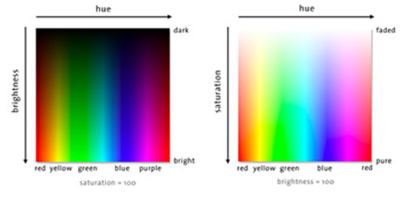
\includegraphics[width=0.5\linewidth]{images/colours} 

}

\caption{Hue, brightness and saturation}\label{fig:colours}
\end{figure}

Read more about the model here:
\url{http://ccl.northwestern.edu/netlogo/models/BugHuntCamouflage}

\hypertarget{neutral-or-adaptive-evolution-in-humans}{%
\chapter{Neutral or adaptive evolution in
humans?}\label{neutral-or-adaptive-evolution-in-humans}}

\hypertarget{objective}{%
\section{Objective}\label{objective}}

The objective of this exercise is to develop an intuitive understanding
of the effect of selection and genetic drift on traits.

\hypertarget{background}{%
\section{Background}\label{background}}

Traits that are under moderate or strong selection will tend to be
restricted to some optimal value, or change directionally -- natural
selection leading to adaptive evolution. Traits that are under weak or
no selection will not be restricted so much so will tend to change via a
random process -- random genetic drift leading to neutral evolution.
Both of these changes require the existence of variation in the trait to
begin with: if there is no, or very little, variation the trait will not
respond much even if there is strong selection.

Finally, the strength of selection will largely depend on the
environment. Traits may be important in some environments but not
others. There may also be traits that would be selected for in some
environments, but against in others. E.g. production of the skin
pigment, melanin, would be selected for in areas with high UV-radiation
since it protect against skin cancer, but selected against in cool
temperate zones with low UV radiation since it inhibits the ability to
make vitamin D (deficiency is a health risk).

\begin{figure}

{\centering 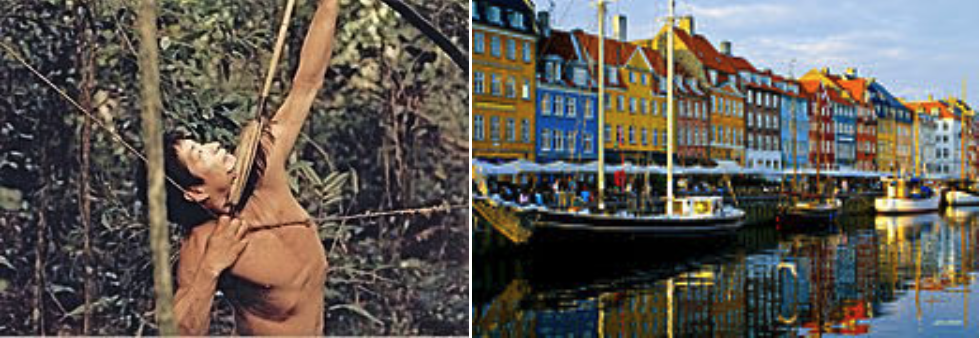
\includegraphics[width=0.5\linewidth]{images/huntergathererDK} 

}

\caption{How will selection differ between these environments?}\label{fig:huntergatherer}
\end{figure}

\hypertarget{your-task}{%
\section{Your task}\label{your-task}}

You are given a list of traits for humans (below). In small groups,
write the traits onto PostIt notes. Then discuss them and place the
traits in order of strength of natural selection that you think would be
acting on the traits in hunter-gatherer-type societies. These
populations are likely to be experiencing the conditions that humans
have experienced over most of our time as a species.

This should result in an ordering of the traits from ones which would
evolve only by the neutral process of \textbf{GENETIC DRIFT} and ones
that would evolve by \textbf{ADAPTIVE EVOLUTION} via \textbf{NATURAL
SELECTION}.

Now repeat this exercise for humans in modern industrialised countries
like Denmark.

\hypertarget{the-traits}{%
\section{The traits}\label{the-traits}}

\hypertarget{hardy-weinberg-equilibrium}{%
\chapter{Hardy-Weinberg equilibrium}\label{hardy-weinberg-equilibrium}}

\hypertarget{problem-1.}{%
\section{Problem \#1.}\label{problem-1.}}

You have sampled a population in which you know that the percentage of
the homozygous recessive genotype (aa) is 36\%. Using that 36\%,
calculate the following: * The frequency of the ``aa'' genotype. * The
frequency of the ``a'' allele. * The frequency of the ``A'' allele. *
The frequencies of the genotypes ``AA'' and ``Aa.'' * The frequencies of
the two possible phenotypes if ``A'' is completely dominant over ``a.''

\hypertarget{problem-2.}{%
\section{Problem \#2.}\label{problem-2.}}

Sickle-cell anemia is an interesting genetic disease. Normal homozygous
individials (SS) have normal blood cells that are easily infected with
the malarial parasite. Thus, many of these individuals become very ill
from the parasite and many die. Individuals homozygous for the
sickle-cell trait (ss) have red blood cells that readily collapse when
deoxygenated. Although malaria cannot grow in these red blood cells,
individuals often die because of the genetic defect. However,
individuals with the heterozygous condition (Ss) have some sickling of
red blood cells, but generally not enough to cause mortality. In
addition, malaria cannot survive well within these ``partially
defective'' red blood cells. Thus, heterozygotes tend to survive better
than either of the homozygous conditions.

\begin{itemize}
\tightlist
\item
  If 9\% of an African population is born with a severe form of
  sickle-cell anemia (ss), what percentage of the population will be
  more resistant to malaria because they are heterozygous (Ss) for the
  sickle-cell gene?
\end{itemize}

\hypertarget{problem-3.}{%
\section{Problem \#3.}\label{problem-3.}}

There are 100 students in a class. Ninety-six did well in the course
whereas four blew it totally and received a grade of F. In the highly
unlikely event that these traits are genetic rather than environmental,
if these traits involve dominant and recessive alleles, and if the four
(4\%) represent the frequency of the homozygous recessive condition,
please calculate the following:

\begin{itemize}
\tightlist
\item
  The frequency of the recessive allele.
\item
  The frequency of the dominant allele.
\item
  The frequency of heterozygous individuals.
\end{itemize}

\hypertarget{problem-4.}{%
\section{Problem \#4.}\label{problem-4.}}

Within a population of butterflies, the color brown (B) is dominant over
the color white (b). And, 40\% of all butterflies are white. Given this
simple information calculate the following:

\begin{itemize}
\tightlist
\item
  The percentage of butterflies in the population that are heterozygous.
\item
  The frequency of homozygous dominant individuals.
\end{itemize}

\hypertarget{how-many-eggs-should-a-bird-lay}{%
\chapter{How many eggs should a bird
lay?}\label{how-many-eggs-should-a-bird-lay}}

\hypertarget{objectives}{%
\section{Objectives}\label{objectives}}

The objective of this exercise is to get an understanding the trade off
between the benefits of producing large numbers of offspring and the
costs of reduced survival of those offspring. This is known as ``Lack's
clutch size.''

\hypertarget{background-1}{%
\section{Background}\label{background-1}}

David Lack was a British ornithologist who proposed that the number of
eggs a bird should lay was the result of a trade-off between the
benefits of producing large numbers of offspring, and the survival costs
of feeding the chicks that hatch.

In other words, although it is beneficial in fitness terms to have many
offspring, the survival of those offspring will decline if they cannot
be cared for.

\hypertarget{your-task-1}{%
\section{Your task}\label{your-task-1}}

The big bird (\emph{Bigus canarius}) (Fig @ref(fig:bigbird)) can lay up
to 10 eggs per breeding season. If there is only 1 egg, the probability
that the parents can adequately feed the chick and ensure it survives is
very high (0.9). However, as the number of siblings increases, the
amount of energy and food that the parents can dedicate to caring for
\emph{each} chick decreases, and the probability of survival therefore
declines . With a clutch size of 10 eggs, there is so little food
\emph{per chick} that the survival rates are close to zero.

\begin{figure}

{\centering 
\includegraphics[width=0.5\linewidth]{images/bigbird} 

}

\caption{Big bird, *Bigus canarius*}\label{fig:bigbird}
\end{figure}

A recent study gathered data on chick survival probability as a function
of number of eggs in the nest. These are given in the table below.

Use these data to plot a graph in Excel with number of eggs on the
x-axis and survival probability on the y-axis axis.

Now, in another column in Excel, calculate, given the chick survival
probability, what the expected number of surviving chicks will be for a
big bird laying between 1 and 10 eggs\footnote{This may require some
  thought!}.

Plot your result on another graph with number of eggs on the x-axis and
number of surviving offspring on the y-axis.

What do you notice? What is the optimum number of eggs to lay?

Advanced: What happens to the optimum as you change the relationship
between clutch size and survival.

\hypertarget{trade-offs-and-the-force-of-selection}{%
\chapter{Trade-offs and the force of
selection}\label{trade-offs-and-the-force-of-selection}}

Why does evolution `care' less and less about you as you age? Because
there are trade-offs between early and late life events.

\hypertarget{objective-1}{%
\section{Objective}\label{objective-1}}

The aim of this exercise is to gain an understanding of early-life
late-life trade offs. Specifically it is to understand why events early
in life tend to be much more important to evolution than those that
happen later in life.

\hypertarget{background-2}{%
\section{Background}\label{background-2}}

An important kind of trade off are those which occur between early and
late life. For example, it may be beneficial to increase reproduction at
younger ages, but this might lead to increased risk of death at older
ages. A mechanism for this could be that limited resources are allocated
to producing offspring rather than maintaining/repairing the body.
Methods

Open the Excel file
\href{https://www.dropbox.com/s/7eyoencvqc3hwv7/TradeOffsAndForceOfSelection.xlsx?dl=1}{TradeOffsAndForceOfSelection.xlsx}.

This file shows a simplified life table, following a cohort of 1000
individuals for a fictional creature.

Survival rates from year to year are set to be 0.8 (i.e.~80\% make it
through to the next year). This fixed, constant survival rate leads to
an exponentially declining survival curve, illustrated with a chart in
the Excel file. Fertility (i.e.~the number of babies produced per year)
is set to be 10 per year.

The product of survival (\(l_x\)) and fertility (\(m_x\)), lxmx is a
measure of the expected number of offspring in an age class. For a
stable population the sum of these values (\(\sum l_x m_x\)) is a
measure of net population growth rate (also known as \(R_0\)). \(R_0\)
is an excellent measure of fitness of a life history strategy.

Note that the initial \(R_0\) is 49.811

\hypertarget{exploring-different-life-history-strategies}{%
\section{Exploring different life history
strategies}\label{exploring-different-life-history-strategies}}

\textbf{We will now use this data to explore how alternative life
history strategies affect fitness.}

Consider a trade-off between early reproduction and late life survival
(i.e.~via resources allocated to body maintenance). In this scenario the
species could increase reproduction early in life by allocating more
energy to making babies. However, resources are limited and this will
come at the expense of survival at a later date. A mechanism for this
could be that the body no longer fixes cancers so effectively.

\begin{itemize}
\item
  Simulate this by adding 1 to fertility (\(m_x\)) in year 1 (the
  benefit) but reducing survival to 0 (all die) at age 25 (the cost).
  \emph{What is the fitness of this strategy?}
\item
  By setting survival to 0 at other ages, determine how many years of
  life could be lost before this cost is no longer worth bearing. Is
  this surprising?
\item
  Now reset everything (\(m_x\) =10; survival = 0.8). Recall what
  fitness was when you added 1 to \(m_x\) at age 1 (50.811).
\item
  If, instead of adding to \(m_x\) at age 1 you were to increase \(m_x\)
  at age 25, how much would you need to increase \(m_x\) to to reach
  this figure?
\item
  What about at age 20? Age 15? Age 10? Age 5? Plot the increase
  required vs.~age (make a new worksheet/ark in Excel) What do you
  notice?
\item
  Reset everything again (\(m_x\) =10; survival = 0.8). Set \(m_x\) from
  age 15 onwards to be 0. Now alter survival rate after this point (at
  ages 15-25). What happens to fitness?
\end{itemize}

\hypertarget{making-a-phylogeny}{%
\chapter{Making a phylogeny}\label{making-a-phylogeny}}

{[}coming soon{]}

\hypertarget{short-answer-exam-discussion}{%
\chapter{Short answer exam
discussion}\label{short-answer-exam-discussion}}

{[}coming soon{]}

\hypertarget{the-red-queen-game}{%
\chapter{The Red Queen Game}\label{the-red-queen-game}}

{[}coming soon{]}

\hypertarget{part-solutions-to-exercises}{%
\chapter*{(PART) Solutions to
exercises}\label{part-solutions-to-exercises}}
\addcontentsline{toc}{chapter}{(PART) Solutions to exercises}

\hypertarget{solutions-and-take-home-messages}{%
\chapter{Solutions and ``take-home''
messages}\label{solutions-and-take-home-messages}}

In this section you will find the solutions and/or main take home
messages of the practical exercises used in this course.

\hypertarget{solutions-bug-hunt-camouflage}{%
\section{Solutions: Bug hunt
camouflage}\label{solutions-bug-hunt-camouflage}}

\begin{itemize}
\tightlist
\item
  \emph{What happens to the average colour of the bug population with
  time as you hunt?}
\end{itemize}

The colour evolves to become more similar to the background colour
because you (the hunter) find it harder to find these better-camouflaged
individuals.

\begin{itemize}
\tightlist
\item
  \emph{What happens to your hunting efficiency?}
\end{itemize}

Your hunting efficiency tends to decrease with time because the bugs are
evolving to be harder to see. They are evolving camouflaged colours.

\begin{itemize}
\tightlist
\item
  \emph{Would you say that the bug population becomes worse or better
  adapted to their environment?}
\end{itemize}

The population becomes better-adapted to their environment with time.

\begin{itemize}
\tightlist
\item
  \emph{Can you explain how this happens?}
\end{itemize}

You (the hunter) kill the most obvious bugs first (i.e.~those with
contrasting colours to the background). These are the individuals that
are not well-adapted to the environment. The survivors have offspring
that are similar to them, while the ones you kill leave no offspring. So
as time goes on, the population becomes dominated by individuals that
are well-camouflaged.

\begin{itemize}
\tightlist
\item
  \emph{After simulating in one environment (e.g.~poppy field) for a few
  minutes, pause then switch to another environment. Are the bugs now
  well- or poorly-adapted to their environment?}
\end{itemize}

Changing the environment means that the individuals are now
porrly-adapted to their environment. This is because the individuals now
find themselves in an environment that they did not evolve in. Their
evolved camouflage does not work so well in a new environment.

\begin{itemize}
\tightlist
\item
  \emph{Do the genotypes of individuals change (e.g.~with individual
  age)?}
\end{itemize}

No, individuals' genotypes are fixed. The change in the population
occurs because of selection of individuals to reproduce. Better-adapted
individuals are more likely to reproduce.

\begin{itemize}
\tightlist
\item
  \emph{Increasing the ``max-mutation-step'' makes bug offspring less
  like their parents. How do you think this will influence the speed of
  adaptation of the bugs?}
\end{itemize}

Increasing the amount of variation in offspring will tend to speed up
adaptation. However, there are limits: too much variation can cause
maladaptation of offspring. For example, if a parent is well-adapted
(perfectly camouflaged), too much variation in offspring could lead to
some offspring being poorly-camouflaged and therefore vulnerable to
predation.

\hypertarget{solutions-neutral-or-adaptive-evolution-in-humans}{%
\section{Solutions: Neutral or adaptive evolution in
humans}\label{solutions-neutral-or-adaptive-evolution-in-humans}}

The take home message here is that whether traits are adaptive or
neutral depends on the environment.

Consider genes that confer entibiotic resistance on bacteria. In the
absence of antibiotics, these genes are not important and are not
selected for. They still evolve (if they vary among individuals and are
inherited), but this evolution is neutral with no selection. On the
other hand, when antibiotics are introduced to the system, those same
genes are strongly selected for and evolution of the genes for
antibiotic resistance is now strongly adaptive. Context matters.

The same is the case for traits in humans. Assuming the the traits vary
among individuals and are inherited, their neutrality or adaptiveness
depends on their effect on fitness. If the traits have strong effects on
fitness then they will be under strong selection but if they have weak
or no effects on fitness they will evolve via neutral evolution.

Example traits that evolve via neutral evolution include fingerprint
structure and iris structure. The detailed structures are not important
to fitness, but are still genetically determined, and inherited.

Traits like muscle strength, running speed may have been important for
fitness when they helped our ancestors obtain food. In those
environments, they would have been under selection and therefore evolve
via adaptive evolution. In more modern times, these selection pressures
are weaker.

\hypertarget{making-a-phylogeny-1}{%
\section{Making a phylogeny}\label{making-a-phylogeny-1}}

{[}coming soon{]}

\hypertarget{short-answer-exam-discussion-1}{%
\section{Short answer exam
discussion}\label{short-answer-exam-discussion-1}}

{[}coming soon{]}

\hypertarget{the-red-queen-game-1}{%
\section{The Red Queen game}\label{the-red-queen-game-1}}

{[}coming soon{]}

\backmatter
\end{document}
